%definira klasu dokumenta 
\documentclass[12pt]{report} 

%prostor izmedu naredbi \documentclass i \begin{document} se zove uvod. U njemu se nalaze naredbe koje se odnose na cijeli dokument

%osnovni LaTex ne može riješiti sve probleme, pa se koriste različiti paketi koji olakšavaju izradu željenog dokumenta
\usepackage[croatian]{babel} 
\usepackage{amssymb}
\usepackage{amsmath}
\usepackage{txfonts}
\usepackage{mathdots}
\usepackage{titlesec}
\usepackage{array}
\usepackage{lastpage}
\usepackage{etoolbox}
\usepackage{tabularray}
\usepackage{color, colortbl}
\usepackage{adjustbox}
\usepackage{geometry}
\usepackage[classicReIm]{kpfonts}
\usepackage{hyperref}
\usepackage{fancyhdr}

\usepackage{float}
\usepackage{setspace}
\restylefloat{table}


\patchcmd{\chapter}{\thispagestyle{plain}}{\thispagestyle{fancy}}{}{} %redefiniranje stila stranice u paketu fancyhdr

%oblik naslova poglavlja
\titleformat{\chapter}{\normalfont\huge\bfseries}{\thechapter.}{20pt}{\Huge}
\titlespacing{\chapter}{0pt}{0pt}{40pt}


\linespread{1.3} %razmak između redaka

\geometry{a4paper, left=1in, top=1in,}  %oblik stranice

\hypersetup{ colorlinks, citecolor=black, filecolor=black, linkcolor=black,	urlcolor=black }   %izgled poveznice


%prored smanjen između redaka u nabrajanjima i popisima
\newenvironment{packed_enum}{
	\begin{enumerate}
		\setlength{\itemsep}{0pt}
		\setlength{\parskip}{0pt}
		\setlength{\parsep}{0pt}
	}{\end{enumerate}}

\newenvironment{packed_item}{
	\begin{itemize}
		\setlength{\itemsep}{0pt}
		\setlength{\parskip}{0pt}
		\setlength{\parsep}{0pt}
	}{\end{itemize}}




%boja za privatni i udaljeni kljuc u tablicama
\definecolor{LightBlue}{rgb}{0.9,0.9,1}
\definecolor{LightGreen}{rgb}{0.9,1,0.9}

%Promjena teksta za dugačke tablice
\DefTblrTemplate{contfoot-text}{normal}{Nastavljeno na idućoj stranici}
\SetTblrTemplate{contfoot-text}{normal}
\DefTblrTemplate{conthead-text}{normal}{(Nastavljeno)}
\SetTblrTemplate{conthead-text}{normal}
\DefTblrTemplate{middlehead,lasthead}{normal}{Nastavljeno od prethodne stranice}
\SetTblrTemplate{middlehead,lasthead}{normal}

%podesavanje zaglavlja i podnožja

\pagestyle{fancy}
\lhead{Programsko inženjerstvo}
\rhead{$Medicinska rehabilitacija$}
\lfoot{$Proginator$}
\cfoot{stranica \thepage/\pageref{LastPage}}
\rfoot{\today}
\renewcommand{\headrulewidth}{0.2pt}
\renewcommand{\footrulewidth}{0.2pt}


\begin{document} 
	
	
	
	\begin{titlepage}
		\begin{center}
			\vspace*{\stretch{1.0}} %u kombinaciji s ostalim \vspace naredbama definira razmak između redaka teksta
			\LARGE Programsko inženjerstvo\\
			\large Ak. god. 2023./2024.\\
			
			\vspace*{\stretch{3.0}}
			
			\huge Medicinska rehabilitacija\\
			\Large Dokumentacija, Rev.1 % \textit{1 ili 2}\\
			
			\vspace*{\stretch{12.0}}
			\normalsize
			Grupa: Proginator\\
			Voditelj: Ema Badurina\\
			
			
			\vspace*{\stretch{1.0}}
			Datum predaje: 17. studenog 2023.%\textit{$<$dan$>$. $<$mjesec$>$. $<$godina$>$.}\\
	
			\vspace*{\stretch{4.0}}
			
			Nastavnik: Miljenko Krhen\\
		
		\end{center}

	
	\end{titlepage}

	
	\tableofcontents


	\chapter{Dnevnik promjena dokumentacije}
		
		\textbf{\textit{Kontinuirano osvježavanje}}\\
				
		
		\begin{longtblr}[
				label=none
			]{
				width = \textwidth, 
				colspec={|X[2]|X[10]|X[5]|X[3]|}, 
				rowhead = 1
			}
			\hline
			\textbf{Rev.}	& \textbf{Opis promjene/dodatka} & \textbf{Autori} & \textbf{Datum}\\[3pt] \hline
			0.1 & Dovršen opis projektnog zadatka & E.Badurina & 13.11.2023. 		\\[3pt] \hline 
			0.2	& Dovršen opis arhitekture & L.Lasović & 13.11.2023. 	\\[3pt] \hline 
			0.2.1 & Dodan dio obrazaca uporabe & L.Lasović, E.Badurina & 13.11.2023. \\[3pt] \hline
			0.3 & Dodani svi obrasci uporabe & L.Lasović, E.Badurina & 14.11.2023. \\[3pt] \hline
			0.3.1 & Dodani dijagrami obrazaca uporabe & A.Jakovčević & 14.11.2023. \\[3pt] \hline
			0.3.2 & Revizija i promjene na obrascima uporabe & A.Jakovčević, E.Badurina & 15.11.2023. \\[3pt] \hline
			0.4 & Dodani sekvencijski dijagrami & L.Lasović, E.Badurina & 15.11.2023. \\[3pt] \hline
			0.4.1 & Dodan opis baze & L.Lasović & 15.11.2023. \\[3pt] \hline
			0.4.1 & Ispravak sekvencijskih dijagrama i ostali zahtjevi & E.Badurina & 16.11.2023. \\[3pt] \hline
			\textbf{1.0} & Verzija samo s bitnim dijelovima za 1. ciklus & * & 17.11.2023. \\[3pt] \hline 
			1.1 & * & * \newline * & * \\[3pt] \hline 
			1.2 & * & * & * \\[3pt] \hline  
			\textbf{2.0} & *  & * & * \\[3pt] \hline 
			&  &  & \\[3pt] \hline	
		\end{longtblr}
	
	
		\textit{Moraju postojati glavne revizije dokumenata 1.0 i 2.0 na kraju prvog i drugog ciklusa. Između tih revizija mogu postojati manje revizije već prema tome kako se dokument bude nadopunjavao. Očekuje se da nakon svake značajnije promjene (dodatka, izmjene, uklanjanja dijelova teksta i popratnih grafičkih sadržaja) dokumenta se to zabilježi kao revizija. Npr., revizije unutar prvog ciklusa će imati oznake 0.1, 0.2, …, 0.9, 0.10, 0.11.. sve do konačne revizije prvog ciklusa 1.0. U drugom ciklusu se nastavlja s revizijama 1.1, 1.2, itd.}
	
\chapter{Opis projektnog zadatka}
		
		\textbf{\textit{dio 1. revizije}}\\
		
		
		Cilj ovog projekta je izgradnja web aplikacije koja će omogućiti ljudima/bolesnicima lakše prijavljivanje na slobodne termine za medicinsku rehabilitaciju i fizikalnu terapiju te praćenje njihovog zdravstvenog napretka. Također će omogućiti zaposlenicima ustanove da odbijaju ili prihvaćaju termine ovisno o raspoloživosti prostorija, opreme i osoblja pritom imajući mogućnost uvida u pacijentove prošle terapije i napredak. Vrijeme porovođenja rehabilitacije je svakim radnim danom od ponedjeljka do petka od 8:00 do 20:00 sati.
		
		\noindent Aplikacija će razlikovati tri vrste korisnika: 
		\begin{packed_item}
			
			\item  pacijenta/bolesnika
			\item  liječnika - djelatnika zdravstvene ustanove
			\item  administratora
		\end{packed_item}
		
		Prilikom pokretanja web aplikacije svaki korisnik unosi svoj e-mail i lozinku. Ovisno o vrsti korisnika biti će preusmjereni na različite stranice.
		
		\textit{Pacijent} se samostalno prijavljuje u sustav. U slučaju da još ne postoji imati će opciju registracije. Za registraciju mora unijeti: 
		\begin{packed_item}
			\item ime
			\item prezime
			\item e-mail adresu
			\item MBO - Matični Broj Osiguranika
			\item broj telefona
			\item lozinku
		\end{packed_item}
		Prilikom registracije pomoću MBO-a provjerava se ako korisnik postoji u središnjem informacijskom sustavu zdravstvene zaštite.
		Nakon prijave ili registracije korisnik je preusmjeren na stranicu gdje se prikazuju njegovi termini i zahtjevi. U terminima se prikazuju protekli i budući termini, za protekle termine piše ako je pacijent došao te komentari djelatnika ustanove o napretku. Termin se dobiva nakon što se odobri zahtjev za jednim.		
		Zahtjev se sastoji od:
		\begin{packed_item}
			\item vremena predaje
			\item željenog termina
			\item vrste/tipa rehabilitacije
			\item liječnika koji je uputio pacijenta na terapiju
			\item reference na prošlu terapiju
			\item statusa
		\end{packed_item}
		Status može biti odobreno, odbijeno, čeka na odobrenje ili isteklo u slučaju da nitko nije odobrio niti odbio termin do željenog vremena terapije.
		Klikom na opciju \textit{naruči se} pacijent može napraviti novi zahtjev za terminom. Zahtjev popunjava unoseći vrstu rehabilitacije, liječnika koji ga je uputio, ukoliko se radi o ponovljenoj terapiji odabrati će i termin već obavljenog postupka terapije u ustanovi, također u komentar za liječnika dodaje opis svojih oboljenja. Status liječnika koji je izdao uputnicu provjerava se u imeniku liječnika. U odabiru termina biti će prikazano prvih nekoliko slobodnih termina za odabrani tip rehabilitacije i opcije da se unese željeni datum i vrijeme. Nakon odabira željenog termina pacijent predaje zahtjev. Pacijent će o odobrenju ili odbijanju zahtjeva, kao i svim mogućim promjenama biti obaviješten mailom.
		
		\textit{Liječnik} nakon prijavljivanja u sustav ima pregled svih pacijenata i njihovih podataka, klikom na prikaz terapije bit će mu prikazani svi termini odabranog pacijenta i detalji o njima, tu će imati opciju evidentirati dolazak pacijenta i zabilježiti komentare vezane uz napredak ili pregledati napredak i komentare iz prošlih termina. Također svaki djelatnik ustanove imati će mogućnost prihvaćanja ili odbijanja termina ovisno o raspoloživosti prostorija i opreme. Liječnik koji prihvati zahtjev automatski će se dodati kao liječnik koji će tu terapiju izvoditi. 
		
		\textit{Administrator} ima pregled svih pacijenata i djelatnika. Uz ovlasti koje imaju djelatnici administrator pri zaposlenju novog liječnika izrađuje korisnički račun za njega s inicijalnom lozinkom. Također nakon prestanka radnog odnosa administrator može ukloniti tog liječnika. Administrator definira sve što je potrebno za ispravan rad sustava, dakle može mijenjati broj opreme, dostupne prostorije.
		
		Ovim projektom smanjio bi se opseg posla djelatnika ustanove 
		---
		
		Aplikacija će se moći proširiti da djelatnici uopće ne moraju prihvaćati ili odbijati prijave, već će to sustav raditi automatski na temelju raspoloživih podataka o opremi, prostorijama, djelatnicima i već zauzetim terminima. Svi termini, prostorije, oprema i djelatnici vidljivi su adminu koji im može mijenjati status za određeno vrijeme, na primjer kada liječnik ode na godišnji odmor može promijeniti njegov status u neaktivan za to razdoblje ili kada cijela ustanova ima sastanak onemogućiti sve termine za vrijeme tog sastanka. Ostala bi mogućnost upućivanja maila ili telefonskog poziva pacijentu u slučaju ikakvih promjena. 
		
		
		---
		
	
		
		\begin{packed_item}
			\item \textit{potencijalna korist ovog projekta}
			\item \textit{postojeća slična rješenja (istražiti i ukratko opisati razlike u odnosu na zadani zadatak). Dodajte slike koja predočavaju slična rješenja.}
			\item \textit{skup korisnika koji bi mogao biti zainteresiran za ostvareno rješenje.}
			\item \textit{mogućnost prilagodbe rješenja }
			\item \textit{opseg projektnog zadatka}
			\item \textit{moguće nadogradnje projektnog zadatka}
		\end{packed_item}
		
		\textit{Za pomoć pogledati reference navedene u poglavlju „Popis literature“, a po potrebi konzultirati sadržaj na internetu koji nudi dobre smjernice u tom pogledu.}
		\eject
		
		\section{Primjeri u \LaTeX u}
		
		\textit{Ovo potpoglavlje izbrisati.}\\

		U nastavku se nalaze različiti primjeri kako koristiti osnovne funkcionalnosti \LaTeX a koje su potrebne za izradu dokumentacije. Za dodatnu pomoć obratiti se asistentu na projektu ili potražiti upute na sljedećim web sjedištima:
		\begin{itemize}
			\item Upute za izradu diplomskog rada u \LaTeX u - \url{https://www.fer.unizg.hr/_download/repository/LaTeX-upute.pdf}
			\item \LaTeX\ projekt - \url{https://www.latex-project.org/help/}
			\item StackExchange za Tex - \url{https://tex.stackexchange.com/}\\
		
		\end{itemize} 	


		
		\noindent \underbar{podcrtani tekst}, \textbf{podebljani tekst}, 	\textit{nagnuti tekst}\\
		\noindent \normalsize primjer \large primjer \Large primjer \LARGE {primjer} \huge {primjer} \Huge primjer \normalsize
				
		\begin{packed_item}
			
			\item  primjer
			\item  primjer
			\item  primjer
			\item[] \begin{packed_enum}
				\item primjer
				\item[] \begin{packed_enum}
					\item[1.a] primjer
					\item[b] primjer
				\end{packed_enum}
				\item primjer
			\end{packed_enum}
			
		\end{packed_item}
		
		\noindent primjer url-a: \url{https://www.fer.unizg.hr/predmet/proinz/projekt}
		
		\noindent posebni znakovi: \# \$ \% \& \{ \} \_ 
		$|$ $<$ $>$ 
		\^{} 
		\~{} 
		$\backslash$ 
		
		
		\begin{longtblr}[
			label=none,
			entry=none
			]{
				width = \textwidth,
				colspec={|X[8,l]|X[8, l]|X[16, l]|}, 
				rowhead = 1,
			} %definicija širine tablice, širine stupaca, poravnanje i broja redaka naslova tablice
			\hline \SetCell[c=3]{c}{\textbf{naslov unutar tablice}}	 \\ \hline[3pt]
			\SetCell{LightGreen}IDKorisnik & INT	&  	Lorem ipsum dolor sit amet, consectetur adipiscing elit, sed do eiusmod  	\\ \hline
			korisnickoIme	& VARCHAR &   	\\ \hline 
			email & VARCHAR &   \\ \hline 
			ime & VARCHAR	&  		\\ \hline 
			\SetCell{LightBlue} primjer	& VARCHAR &   	\\ \hline 
		\end{longtblr}
		

		\begin{longtblr}[
				caption = {Naslov s referencom izvan tablice},
				entry = {Short Caption},
			]{
				width = \textwidth, 
				colspec = {|X[8,l]|X[8,l]|X[16,l]|}, 
				rowhead = 1,
			}
			\hline
			\SetCell{LightGreen}IDKorisnik & INT	&  	Lorem ipsum dolor sit amet, consectetur adipiscing elit, sed do eiusmod  	\\ \hline
			korisnickoIme	& VARCHAR &   	\\ \hline 
			email & VARCHAR &   \\ \hline 
			ime & VARCHAR	&  		\\ \hline 
			\SetCell{LightBlue} primjer	& VARCHAR &   	\\ \hline 
		\end{longtblr}
	


		
		
		%unos slike
		\begin{figure}[H]
			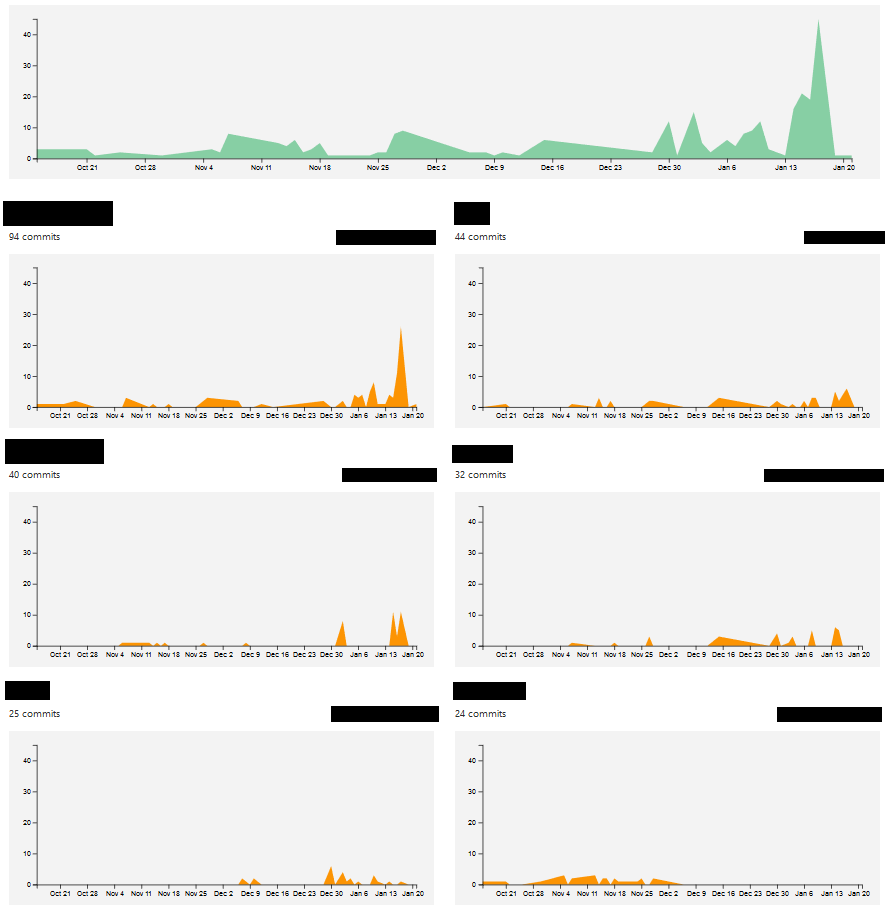
\includegraphics[scale=0.4]{slike/aktivnost.PNG} %veličina slike u odnosu na originalnu datoteku i pozicija slike
			\centering
			\caption{Primjer slike s potpisom}
			\label{fig:promjene}
		\end{figure}
		
		\begin{figure}[H]
			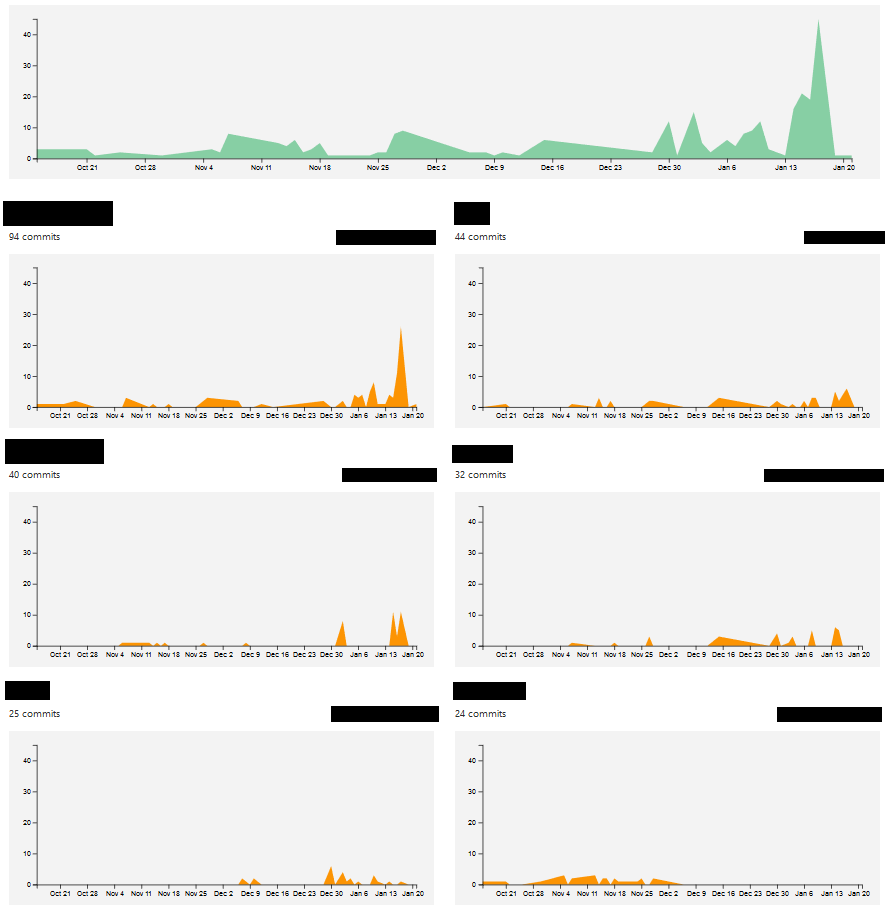
\includegraphics[width=\textwidth]{slike/aktivnost.PNG} %veličina u odnosu na širinu linije
			\caption{Primjer slike s potpisom 2}
			\label{fig:promjene2} %label mora biti drugaciji za svaku sliku
		\end{figure}
		
		Referenciranje slike \ref{fig:promjene2} u tekstu.
		
		\eject
		
	
	\chapter{Specifikacija programske potpore}
		
	\section{Funkcionalni zahtjevi}			
			
			\noindent \textbf{Dionici:}
			
			\begin{packed_enum}
				
				\item Pacijent
				\item Djelatnik	
				\begin{packed_item}
					\item Liječnik
					\item Administrator
				\end{packed_item}
				\item Razvojni tim
				
			\end{packed_enum}
			
			Pacijenti i djelatnici zajedničkim imenom su korisnici.
			
			
			\noindent \textbf{Aktori i njihovi funkcionalni zahtjevi:}
			
			
			\begin{packed_enum}
				\item  \underbar{Neregistrirani korisnik (inicijator) može:}
				\begin{packed_enum}
					\item registrirati se u sustav, unijeti potrebne podatke(ime, prezime, e-mail adresu, MBO, broj telefona, lozinku)
				\end{packed_enum}
			
				\item  \underbar{Neprijavljeni korisnik (inicijator) može:}
				\begin{packed_enum}
					\item prijaviti se u sustav koristeći svoju e-mail adresu i lozinku
				\end{packed_enum}
				
				\item  \underbar{Pacijent-\textit{prijavljeni korisnik} (inicijator) može:}
				\begin{packed_enum}
					\item prikazati i mijenjati svoje osobne podatke i lozinku
					\item vidjeti svoje zahtjeve za terminom terapije (vrijeme predaje zahtjeva, vrijeme željenog termina, tip rehabilitacije, liječnika koji ga je uputio na rehabilitaciju, referencu na prošlu terapiju i status) 
					\item vidjeti svoje termine (vrijeme termina, prostoriju, tip rehabilitacije, liječnika, napomene i ishod termina) 
					\item filtrirati svoje termine
					\item prikazati nalaz (detalji i komentari) s termina odrađene terapije
					\item naručiti se na terapiju, unijeti tip rehabilitacije, liječnika koji ga je uputio na terapiju, opis oboljenja i zahtijevani postupak liječenja
					\item odabrati termin za neku terapiju između priloženih ili unijeti datum i odabrati neki na temelju toga ponuđeni termin
				\end{packed_enum}
				
				\item  \underbar{Djelatnik-\textit{prijavljeni korisnik} (inicijator) može:}
				\begin{packed_enum}
					\item prikazati i mijenjati svoje osobne podatke i lozinku
					\item vidjeti popis svih pacijenata (ime, prezime, MBO, e-mail adresa, broj telefona)
					\item prikazati termine pojedinog pacijenta i prikazati evidenciju termina pojedinog pacijenta
					\item evidentirati dolazak pacijenta na termin, dodati komentar o odrađenom terminu i vidjeti informacije o terapiji
					\item prihvatiti/odbiti zahtjev za terminom na temelju raspoloživih prostorija i opreme 
					
				\end{packed_enum}
				\item  \underbar{Administrator - \textit{prijavljeni korisnik} (inicijator)  može:}
				\begin{packed_enum}
					
					\item vidjeti popis svih djelatnika (ime, prezime, OIB, e-mail adresa)
					\item urediti podatke djelatnika
					\item ukloniti djelatnika
					\item dodati/registrirati novog djelatnika (ime, prezime, e-mail adresa, OIB, lozinka)
					\item mijenjati raspoloživost soba i opreme
					\item dodavati opremu i sobe
					\item otkazivati i mijenjati termine, te o tome obavještavati pacijenta
					
				\end{packed_enum}
				
				\item  \underbar{Baza podataka (sudionik) može:}
				\begin{packed_enum}
					
					\item pohranjuje podatke i ovlasti korisnika
					\item pohranjuje podatke o opremi i prostorijama
					\item pohranjuje podatke o terapijama i terminima
					
				\end{packed_enum}
			\end{packed_enum}
			
			\eject 
			
			
				
			\subsection{Obrasci uporabe}
				
				
				\subsubsection{Opis obrazaca uporabe}
					

					\noindent \underbar{\textbf{UC1 - Prijava u sustav}}
					\begin{packed_item}
	
						\item \textbf{Glavni sudionik: }Korisnik
						\item  \textbf{Cilj: } Prijaviti se u sustav
						\item  \textbf{Sudionici: } Baza podataka
						\item  \textbf{Preduvjet: } Korisnik je registriran u sustav
						\item  \textbf{Opis osnovnog tijeka: }
						
						\item[] \begin{packed_enum}
	
							\item Korisnik unosi svoju e-mail adresu i lozinku
							\item Provjera ispravnosti podataka
							\item Prikaz početne stranice ovisno o korisniku
						\end{packed_enum}
						
						\item  \textbf{Opis mogućih odstupanja:}
						
						\item[] \begin{packed_item}
	
							\item[2.a] Neispravna e-mail adresa ili lozinka
							\item[] \begin{packed_enum}
								
								\item obavijest o neispravnosti unesenih podataka
								
							\end{packed_enum}
							
						\end{packed_item}
					\end{packed_item}
				
				\noindent \underbar{\textbf{UC2 - Registracija}}
				\begin{packed_item}
					
					\item \textbf{Glavni sudionik: }Neregistrirani korisnik
					\item  \textbf{Cilj: }Registrirati se u sustav
					\item  \textbf{Sudionici: }Baza podataka
					\item  \textbf{Preduvjet: } -  
					\item  \textbf{Opis osnovnog tijeka: }
					
					\item[] \begin{packed_enum}
						
						\item Korisnik unosi svoje podatke (ime, prezime, e-mail adresu, MBO, lozinka)
						\item Provjera ispravnosti podataka verifikacijom iz baze podataka sustava zdravstvene zaštite
						\item Prikaz stranice za prijavu u sustav
					\end{packed_enum}
					
					\item  \textbf{Opis mogućih odstupanja:}
					
					\item[] \begin{packed_item}
						
						\item[2.a] Korisnik ne postoji u sustavu zdravstvene zaštite
						\item[] \begin{packed_enum}
							
							\item Sustav obavještava korisnika o neispravnosti podataka
							\item Korisnik mijenja podatke ili odustaje od registracije
							
						\end{packed_enum}
						
					\end{packed_item}
				\end{packed_item}
				
				\noindent \underbar{\textbf{UC3 - pregled osobnih podataka}}
				\begin{packed_item}
					
					\item \textbf{Glavni sudionik: }Korisnik
					\item  \textbf{Cilj: }Pregledati osobne podatke 
					\item  \textbf{Sudionici: }Baza podataka
					\item  \textbf{Preduvjet: }Korisnik mora biti prijavljen u sustav
					\item  \textbf{Opis osnovnog tijeka: }
					
					\item[] \begin{packed_enum}
						
						\item Korisnik odabire opciju "Profil"
						\item Sustav prikazuje korisnikove osobne podatke 
					\end{packed_enum}
					
				\end{packed_item}
				\noindent \underbar{\textbf{UC4 - Promjena osobnih podataka}}
				\begin{packed_item}
					
					\item \textbf{Glavni sudionik: }Korisnik
					\item  \textbf{Cilj: }Promijeniti osobne podatke
					\item  \textbf{Sudionici: }Baza podataka
					\item  \textbf{Preduvjet: }Korisnik mora biti prijavljen u sustav
					\item  \textbf{Opis osnovnog tijeka: }
					
					\item[] \begin{packed_enum}
						
						\item Korisnik odabire opciju "Uredi"  
						\item Korisnik unosi/mijenja podatke
						\item Korisnik odabire opciju "Spremi promjene"
					\end{packed_enum}
				\end{packed_item}
				
				\noindent \underbar{\textbf{UC5 - Promjena lozinke}}
				\begin{packed_item}
					
					\item \textbf{Glavni sudionik: }Korisnik
					\item  \textbf{Cilj: }Promijeniti lozinku
					\item  \textbf{Sudionici: }Baza podataka
					\item  \textbf{Preduvjet: }Korisnik je prijavljen u sustav
					\item  \textbf{Opis osnovnog tijeka: }
					
					\item[] \begin{packed_enum}
						
						\item Korisnik odabire opciju "Promijeni lozinku"
						\item Korisnik potvrđuje staru lozinku
						\item Korisnik unosi novu lozinku
						\item Korisnik potvrđuje novu lozinku
						\item Sustav korisnika prebacuje na prijavu
						\item Korisnik se prijavljuje s novom lozinkom
					\end{packed_enum}
					
					\item  \textbf{Opis mogućih odstupanja:}
					
					\item[] \begin{packed_item}
						
						\item[2.a] korisnik unosi neispravnu staru lozinku
						\item[] \begin{packed_enum}
							
							\item Sustav upozorava korisnika o neispravnosti lozinke
							\item Korisnik ponovno unosi lozinku ili odustaje od promjene
							
						\end{packed_enum}
						\item[3.a] Nova lozinka je jednaka staroj
						\item[]\begin{packed_enum}
							
							\item Sustav upozorava korisnika da su mu lozinke iste
							\item Korisnik mijenja novu lozinku ili odustaje od promjene
							
						\end{packed_enum}
						
					\end{packed_item}
				\end{packed_item}
				
				\noindent \underbar{\textbf{UC6 - Kreiranje terapije(\ref{fig:sekvencijski_dijagram_1})}}
				\begin{packed_item}
					
					\item \textbf{Glavni sudionik: }Pacjient
					\item  \textbf{Cilj: }Kreiranje procesa terapije
					\item  \textbf{Sudionici: }Baza podataka
					\item  \textbf{Preduvjet: }Pacijent je prijavljen u sustav
					\item  \textbf{Opis osnovnog tijeka: }
					
					\item[] \begin{packed_enum}
						
						\item Pacijent odabire opciju "Kreiraj terapiju"
						\item Otvara se stranica za prijavljivanje terapije
						\item Pacijent unosi ime i prezime liječnika, opis oboljenja i zahtijevani postupak liječenja, te odabire vrstu terapije
						\item Pacijent odabire opciju "Pošalji"
						\item Provjera ispravnosti podataka u imeniku liječnika
						\item Prikaz stranice za odabir termina
					\end{packed_enum}
					
					\item  \textbf{Opis mogućih odstupanja:}
					
					\item[] \begin{packed_item}
						
						\item[3.a] Liječnik ne postoji u imeniku liječnika
						\item[] \begin{packed_enum}
							
							\item Sustav obavještava pacijenta o neispravnim podacima(ime i prezime liječnika)
							\item Pacijent mijenja podatke ili odustaje od kreiranja terapije
							
						\end{packed_enum}
												
					\end{packed_item}
				\end{packed_item}
				\noindent \underbar{\textbf{UC7 - Odabir termina}}
				\begin{packed_item}
					
					\item \textbf{Glavni sudionik: }Pacijent
					\item  \textbf{Cilj: }Poslati zahtjev za željenim terminom
					\item  \textbf{Sudionici: }Baza podataka
					\item  \textbf{Preduvjet: }Pacijent je prijavljen u sustav
					\item  \textbf{Opis osnovnog tijeka: }
					
					\item[] \begin{packed_enum}
						
						\item Pacijent odabire terapiju za koju se prijavljuje na termin
						\item Pacijent unosi datum i na temelju njega bira ponuđene slobodne termine
						\item Pacijent opcionalno dodaje napomenu za liječnika
						\item Pacijent šalje zahtjev klikom na "Pošalji"
						\item Spremanje podataka u bazu i slanje maila s podatcima o terminu
						
					\end{packed_enum}
					
					\item  \textbf{Opis mogućih odstupanja:}
					
					\item[] \begin{packed_item}
						\item[2.a] Pacijentu ne odgovara niti jedan termin
						\item[] \begin{packed_enum}
							
							\item Pacijent odustaje od prijave na termin
							
						\end{packed_enum}
						
					\end{packed_item}
				\end{packed_item}
				
			
				
				\noindent \underbar{\textbf{UC8 - Prikaz nalaza termina}}
				\begin{packed_item}
					
					\item \textbf{Glavni sudionik: }Pacijent
					\item  \textbf{Cilj: }Pacijent vidi svoje nalaze
					\item  \textbf{Sudionici: }Baza podataka
					\item  \textbf{Preduvjet: }Prijavljen u sustav, postoje prošli termini
					\item  \textbf{Opis osnovnog tijeka: }
					
					\item[] \begin{packed_enum}
						
						\item Pacijent odabire opciju prikaži nalaz
						\item Otvara se skočni prozor s informacijama i komentarom liječnika (nalazom)
						\item Pacijent odabire opciju zatvori u skočnom prozoru
					\end{packed_enum}
				\end{packed_item}
				
				\noindent \underbar{\textbf{UC9 - Prikaz pacijenta}}
				\begin{packed_item}
					
					\item \textbf{Glavni sudionik: }Djelatnik
					\item  \textbf{Cilj: }Prikazati termine pojedinog pacijenta 
					\item  \textbf{Sudionici: }Baza podataka
					\item  \textbf{Preduvjet: }Djelatnik je prijavljen u sustav
				
					\item  \textbf{Opis osnovnog tijeka: }
					
					\item[] \begin{packed_enum}
						
						\item Djelatnik pretražuje pacijenta upisom imena i prezimena u tražilicu
						\item Djelatnik odabire opciju "Prikaži termine" pored željenog pacijenta
						\item Sustav otvara tablicu termina odabranog pacijenta
						\item Djelatnik evidentira(UC10)/prikazuje evidenciju(UC8)
						\item Djelatnik odabire opciju povratka na popis pacijenata
					\end{packed_enum}
					
					\item  \textbf{Opis mogućih odstupanja:}
					
					\item[] \begin{packed_item}
						
						\item[1.a] Upisani pacijent ne postoji u sustavu
						\item[] \begin{packed_enum}
							\item Prikaz teksta o ne postojanju pacijenta
							\item Djelatnik mijenja upisano ime i prezime ili odustaje od pretraživanja
							
						\end{packed_enum}
						
					\end{packed_item}
					\item[] \begin{packed_item}
						
						\item[3.a] Odabrani pacijent još nije bio ni na jednoj terapiji
						\item[] \begin{packed_enum}
							\item Prikaz teksta o ne postojanju termina za odabranog pacijenta
							\item Djelatnik odabire opciju povratka na popis pacijenata
											 							
						\end{packed_enum}
						
					\end{packed_item}
				\end{packed_item}
				
				\noindent \underbar{\textbf{UC10 - Evidencija dolaska(\ref{fig:sekvencijski_dijagram_2})}}
				\begin{packed_item}
					
					\item \textbf{Glavni sudionik: }Djelatnik
					\item  \textbf{Cilj: }Evidentirati dolazak pacijenta na termin 
					\item  \textbf{Sudionici: }Baza podataka
					\item  \textbf{Preduvjet: }
					\item[] \begin{packed_enum}
						
						\item[-] Djelatnik je prijavljen u sustav
						\item[-] Pacijent mora imati termin koji nije evidentiran
					\end{packed_enum}
					\item  \textbf{Opis osnovnog tijeka: }
					
					\item[] \begin{packed_enum}
						\item Djelatnik odabire opciju evidentiraj pored termina odabranog pacijenta
						\item Otvara se obrazac za evidenciju dolaska na termin
						\item Djelatnik evidentira dolazak odabirom jedne od tri ponuđene opcije(nije došao, došao je)
						\item Djelatnik unosi komentar o odrađenoj terapiji
						\item Djelatnik predaje evidenciju
						\item Povratak na popis termina odabranog pacijenta
					\end{packed_enum}
					
					\item  \textbf{Opis mogućih odstupanja:}
					
					\item[] \begin{packed_item}
						
						\item[3.a] Djelatnik odustaje od evidentiranja termina
						\item[] \begin{packed_enum}
							\item Djelatnik odabire opciju povratka na popis termina odabranog pacijenta
							
						\end{packed_enum}
					\end{packed_item}
				\end{packed_item}
				
					
				
				\noindent \underbar{\textbf{UC11 - Registracija djelatnika}}
				\begin{packed_item}
					
					\item \textbf{Glavni sudionik: }Administrator
					\item  \textbf{Cilj: }Registrirati novog liječnika
					\item  \textbf{Sudionici: }Baza podataka
					\item  \textbf{Preduvjet: }
					\item[] \begin{packed_enum}
						
						\item[-] Djelatnik je prijavljen u sustav
						\item[-] Djelatnik ima ovlasti administratora
					\end{packed_enum}
					\item  \textbf{Opis osnovnog tijeka: }
					
					\item[] \begin{packed_enum}
						\item Djelatnik odaibre opciju "Dodaj djelatnika"
						\item Prikazuje se stranica za registraciju novog djelatnika
						\item Administrator unosi podatke o djelatniku(ime, prezime, OIB, e-mail adresu i inicijalnu lozinku)
						\item Administrator odabire opciju "Dodaj račun"
						\item Podatci se unose u bazu podataka
					\end{packed_enum}
					
					\item  \textbf{Opis mogućih odstupanja:}
					
					\item[] \begin{packed_item}
						
						\item[3.a] Podatci ne zadovoljavaju željeni format
						\item[] \begin{packed_enum}
							\item Sustav upozorava administratora o neispravnom formatu podataka
							\item Administrator mijenja podatke ili odustaje od registracije djelatnika							
						\end{packed_enum}
					\end{packed_item}
				\end{packed_item}
				
				\noindent \underbar{\textbf{UC12 - Uređivanje podataka djelatnika}}
				\begin{packed_item}
					
					\item \textbf{Glavni sudionik: }Administrator
					\item  \textbf{Cilj: }Promijeniti podatke djelatnika
					\item  \textbf{Sudionici: }Baza podataka
					\item  \textbf{Preduvjet: }
					\item[] \begin{packed_enum}
						
						\item[-] Djelatnik je prijavljen u sustav
						\item[-] Djelatnik ima ovlasti administratora
						\item[-] Postoji barem jedan liječnik/djelatnik
					\end{packed_enum}
					\item  \textbf{Opis osnovnog tijeka: }
					
					\item[] \begin{packed_enum}
						\item Administrator odabire opciju "Uredi" pokraj imena djelatnika
						\item Prikazuje se stranica s podacima odabranog djelatnika
						\item Administrator mijenja podatke o djelatniku(ime, prezime, OIB, e-mail adresu)
						\item Administrator odabire opciju "Spremi"
						\item Podatci se mijenjaju u bazi podataka
						\item Prikazuje se popis djelatnika
					\end{packed_enum}
					
					\item  \textbf{Opis mogućih odstupanja:}
					
					\item[] \begin{packed_item}
						
						\item[3.a] Podatci ne zadovoljavaju željeni format
						\item[] \begin{packed_enum}
							\item Sustav upozorava administratora o neispravnom formatu podataka
							\item Administrator mijenja podatke ili odustaje od promjene podataka							
						\end{packed_enum}
						
						\item[4.a] Administrator ne želi promijeniti podatke 
						\item[] \begin{packed_enum}
							\item Administrator odabire opciju "Odustani"
							\item Podatci se ne mijenjaju u bazi podataka
							\item Prikazuje se popis djelatnika							
						\end{packed_enum}
					\end{packed_item}
				\end{packed_item}
				
				
				\noindent \underbar{\textbf{UC13 - Promjena ovlasti djelatnika}}
				\begin{packed_item}
					
					\item \textbf{Glavni sudionik: }Administrator
					\item  \textbf{Cilj: }Promijeniti ovlasti djelatnika
					\item  \textbf{Sudionici: }Baza podataka
					\item  \textbf{Preduvjet: }
					\item[] \begin{packed_enum}
						
						\item[-] Djelatnik je prijavljen u sustav
						\item[-] Djelatnik ima ovlasti administratora
						\item[-] Postoji barem jedan liječnik/djelatnik
					\end{packed_enum}
					\item  \textbf{Opis osnovnog tijeka: }
					
					\item[] \begin{packed_enum}
						\item Administrator odabire opciju "Uredi" pokraj imena djelatnika
						\item Prikazuje se stranica s podacima odabranog djelatnika
						\item Administrator odabire opciju "Promijeni ovlasti"
						\item Otvara se skočni prozor 
						\item Administrator pridjeljuje/uklanja administratorske ovlasti djelatnika
						\item Administrator odabire opciju "Spremi"
						\item Otvara se skočni prozor s upozorenjem i zahtjevom za unos lozinke administratora
						\item Administrator unosi lozinku
						\item Administrator odabire opcije "potvrdi"
						\item Sustav potvrđuje lozinku i sprema promjene u bazu podataka
						\item Vraća se na podatke o djelatniku
					\end{packed_enum}
					
					\item  \textbf{Opis mogućih odstupanja:}
					
					\item[] \begin{packed_item}
						
						\item[10.a] Administrator je unio neispravnu lozinku
						\item[] \begin{packed_enum}
							\item Sustav upozorava administratora o unosu neispravne lozinke 
							\item Administrator ponovno unosi lozinku ili odustaje od promjene ovlasti						
						\end{packed_enum}
				\end{packed_item}
			\end{packed_item}
				
				\noindent \underbar{\textbf{UC14 - Uklanjanje djelatnika}}
				\begin{packed_item}
					
					\item \textbf{Glavni sudionik: }Administrator
					\item  \textbf{Cilj: }Ukloniti djelatnika
					\item  \textbf{Sudionici: }Baza podataka
					\item  \textbf{Preduvjet: }
					\item[] \begin{packed_enum}
						
						\item[-] Djelatnik je prijavljen u sustav
						\item[-] Djelatnik ima ovlasti administratora
						\item[-] Postoji barem jedan liječnik/djelatnik
					\end{packed_enum}
					\item  \textbf{Opis osnovnog tijeka: }
					
					\item[] \begin{packed_enum}
						\item Administrator odabire opciju "Ukloni" pokraj imena djelatnika
						\item Otvara se skočni prozor s upozorenjem i zahtjevom za unos lozinke administratora
						\item Administrator unosi lozinku
						\item Administrator odabire opciju "Potvrdi"
						\item Sustav potvrđuje lozinku
						\item U bazi podataka se mijenja vrijednost atributa jeAktivan odabranog djelatnika
						\item prikazuje se popis djelatnika bez upravo uklonjenog djelatnika
					\end{packed_enum}
					
					\item  \textbf{Opis mogućih odstupanja:}
					
					\item[] \begin{packed_item}
						
						\item[5.a] Administrator je unio neispravnu lozinku
						\item[] \begin{packed_enum}
							\item Sustav upozorava administratora o unosu neispravne lozinke 
							\item Administrator ponovno unosi lozinku ili odustaje od uklanjanja djelatnika					
						\end{packed_enum}
					\end{packed_item}
				\end{packed_item}
					
					
					\noindent \underbar{\textbf{UC15 - Unos opreme}}
					\begin{packed_item}
						
						\item \textbf{Glavni sudionik: }Administrator
						\item  \textbf{Cilj: }Unos opreme
							\item  \textbf{Sudionici: }Baza podataka
							\item  \textbf{Preduvjet: }
							\item[] \begin{packed_enum}
								
								\item[-] Djelatnik je prijavljen u sustav
								\item[-] Djelatnik ima ovlasti administratora
							\end{packed_enum}
							\item  \textbf{Opis osnovnog tijeka: }
							
							\item[] \begin{packed_enum}
								\item Administrator odabire opciju "Inventar"
								\item Otvara se stranica s popisom opreme
								\item Administrator odabire opciju "Dodaj opremu"
								\item Otvara se skočni prozor s prostorom za unos podataka o opremi
								\item Unosi podatke o opremi (ime i opis)
								\item Odabire prostoriju u kojoj će se oprema nalaziti
								\item Administrator odabire opciju "Spremi"
								\item Podatci se spremaju u bazu podataka i generira se jedinstveni identifikator opreme
								\item Prikazuje se stranica s popisom opreme
							\end{packed_enum}
							
							\item  \textbf{Opis mogućih odstupanja:}
							
							\item[] \begin{packed_item}
								
								\item[6.a] Administrator želi odustati od unosa opreme 
								\item[] \begin{packed_enum}
									\item 	Administrator odabire opciju "odustani"			
								\end{packed_enum}
							\end{packed_item}
						\end{packed_item}
				
				
				\noindent \underbar{\textbf{UC16 - Promjena dostupnosti opreme}}
				\begin{packed_item}
					
					\item \textbf{Glavni sudionik: }Administrator
					\item  \textbf{Cilj: }Promjeniti dostupnost opreme
					\item  \textbf{Sudionici: }Baza podataka
					\item  \textbf{Preduvjet: }
					\item[] \begin{packed_enum}
						
						\item[-] Djelatnik je prijavljen u sustav
						\item[-] Djelatnik ima ovlasti administratora
					\end{packed_enum}
					\item  \textbf{Opis osnovnog tijeka: }
					
					\item[] \begin{packed_enum}
						\item Administrator odabire opciju "Inventar"
						\item Otvara se stranica s popisom opreme
						\item Administrator pretražuje opremu
						\item Administrator mijenja dostupnost opreme odabirom opcije "Dostupno"/"Nedostupno"
						\item Promjena dostupnosti odabrane opreme u bazi podataka
					\end{packed_enum}
					
				\end{packed_item}
				
				\noindent \underbar{\textbf{UC17 - Unos prostorija}}
				\begin{packed_item}
					
					\item \textbf{Glavni sudionik: }Administrator
					\item  \textbf{Cilj: }Unijeti nove prostorije
					\item  \textbf{Sudionici: }Baza podataka
					\item  \textbf{Preduvjet: }
					\item[] \begin{packed_enum}
						
						\item[-] Djelatnik je prijavljen u sustav
						\item[-] Djelatnik ima ovlasti administratora
					\end{packed_enum}
					\item  \textbf{Opis osnovnog tijeka: }
					
					\item[] \begin{packed_enum}
						\item Administrator odabire opciju "Prostorije"
						\item Otvara se stranica s popisom prostorija
						\item Administrator odabire opciju "Dodaj prostoriju"
						\item Prikazuje se skočni prozor s prostorom za unos podataka o prostoriji
						\item Administrator unosi broj i kapacitet prostorije
						\item Administrator odabire opciju "spremi"
						\item Podatci se spremaju u bazu podataka
						\item Prikazuje se stranica s popisom opreme
					\end{packed_enum}
					
					\item  \textbf{Opis mogućih odstupanja:}
					
					\item[] \begin{packed_item}
						
						\item[6.a] Administrator želi odustati od unosa prostorije 
						\item[] \begin{packed_enum}
							\item Administrator odabire opciju "Odustani"
							\end{packed_enum}
					\end{packed_item}
				\end{packed_item}
				
				\noindent \underbar{\textbf{UC18 - Promjena dostupnosti prostorije}}
				\begin{packed_item}
					
					\item \textbf{Glavni sudionik: }Administrator
					\item  \textbf{Cilj: }Promjeniti dostupnost prostorije
					\item  \textbf{Sudionici: }Baza podataka
					\item  \textbf{Preduvjet: }
					\item[] \begin{packed_enum}
						
						\item[-] Djelatnik je prijavljen u sustav
						\item[-] Djelatnik ima ovlasti administratora
					\end{packed_enum}
					\item  \textbf{Opis osnovnog tijeka: }
					
					\item[] \begin{packed_enum}
						\item Administrator odabire opciju "Prostorije"
						\item Otvara se stranica s popisom prostorija
						\item Administrator pretražuje prostorije
						\item Administrator mijenja dostupnost željene prostorije odabirom opcije "Dostupno"/"Nedostupno" koja se nalazi pored podataka o prostoriji
						\item Promjena dostupnosti odabrane prostorije u bazi podataka
					\end{packed_enum}
					
				\end{packed_item}
				
				\noindent \underbar{\textbf{UC19 - Obavijest o promjeni termina}}
				\begin{packed_item}
					
					\item \textbf{Glavni sudionik: }Administrator
					\item  \textbf{Cilj: }Unijeti podatke o novom terminu i obavijestiti pacijenta o tome putem e-maila 
					\item  \textbf{Sudionici: }Baza podataka
					\item  \textbf{Preduvjet: }
					\item[] \begin{packed_enum}
						
						\item[-] Djelatnik je prijavljen u sustav
						\item[-] Djelatnik ima ovlasti administratora
					\end{packed_enum}
					\item  \textbf{Opis osnovnog tijeka: }
					
					\item[] \begin{packed_enum}
						\item Administrator odabire opciju "Promjena termina"
						\item Otvara se stranica s prostorom za podatke o pacijentu i terminu
						\item Administrator pretražuje i odabire pacijenta
						\item Prikazuju se termini odabranog pacijenta koji još nisu evidentirani
						\item Administrator odabire termin koji želi promijeniti
						\item Administrator unosi željene podatke o novom terminu
						\item Prikaz mogućih termina sa željenim podacima
						\item Odabir termina
						\item Administrator opcionalno dodaje komentar
						\item Administrator odabire opciju "Pošalji"
						\item Podaci o terminu se spremaju u bazu podataka
						\item Odabranom pacijentu se šalje e-mail o promjenama i informacijama o novom terminu
					\end{packed_enum}
					
					\item  \textbf{Opis mogućih odstupanja:}
					
					\item[] \begin{packed_item}
						
						\item[3.a] Administrator unosi nepostojećeg pacijenta/krivo uneseno ime/prezime/MBO pacijenta
						\item[] \begin{packed_enum}
							\item Sustav upozorava administratora o nepostojanju pacijenta u sustavu
							\item Administrator mijenja svoj unos ili odustaje od promjene termina
						\end{packed_enum}
					\end{packed_item}
				\end{packed_item}
				
				
				\subsubsection{Dijagrami obrazaca uporabe}
					
					\begin{figure}[H]
						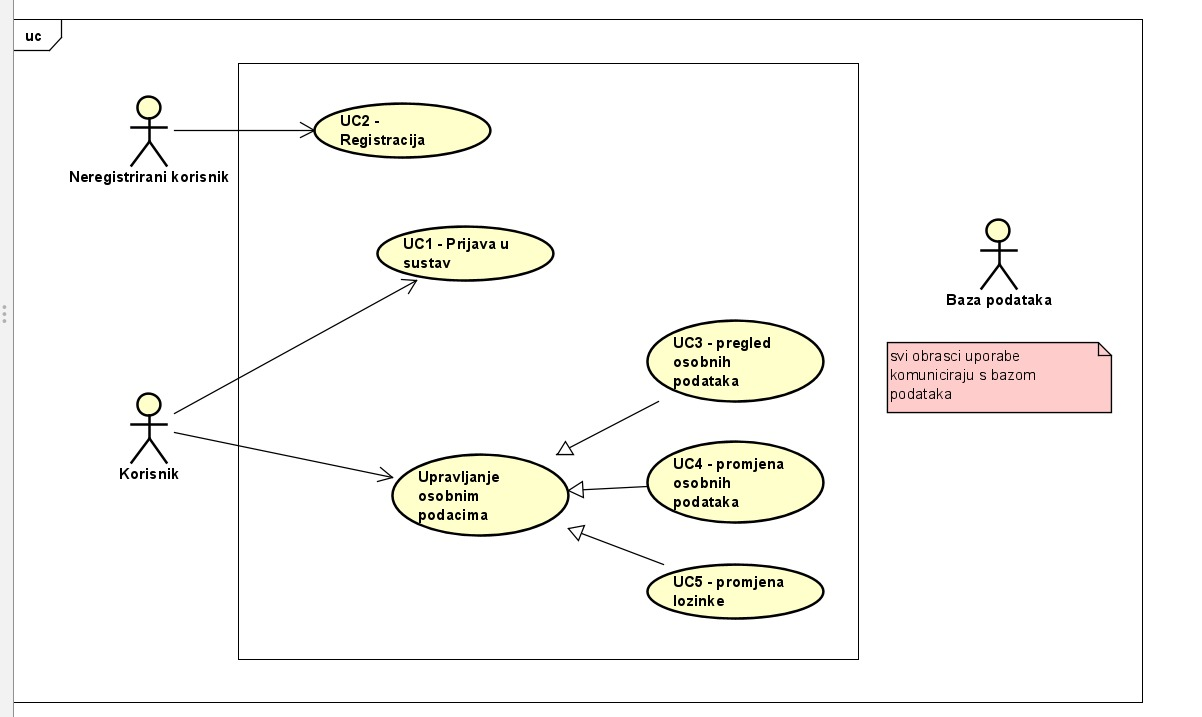
\includegraphics[scale=0.3]{slike/dijagram_obrasca_uporabe1.JPG} %veličina slike u odnosu na originalnu datoteku i pozicija slike
						\centering
						\caption{Dijagram obrasca uporabe - Korisnik i neregistrirani korisnik}
						\label{fig:dijagram_UC1}
					\end{figure}
					
					\begin{figure}[H]
						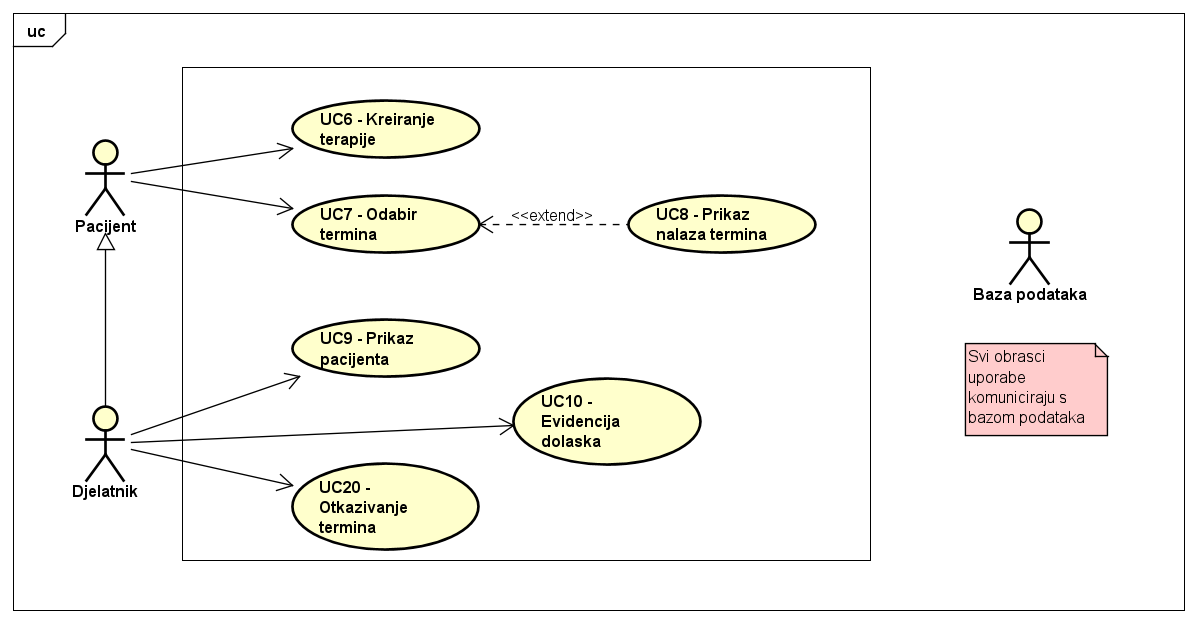
\includegraphics[scale=0.45]{slike/dijagram_obrasca_uporabe2.PNG} %veličina slike u odnosu na originalnu datoteku i pozicija slike
						\centering
						\caption{Dijagram obrasca uporabe - Djelatnik i pacijent}
						\label{fig:dijagram_UC2}
					\end{figure}
					
					\begin{figure}[H]
						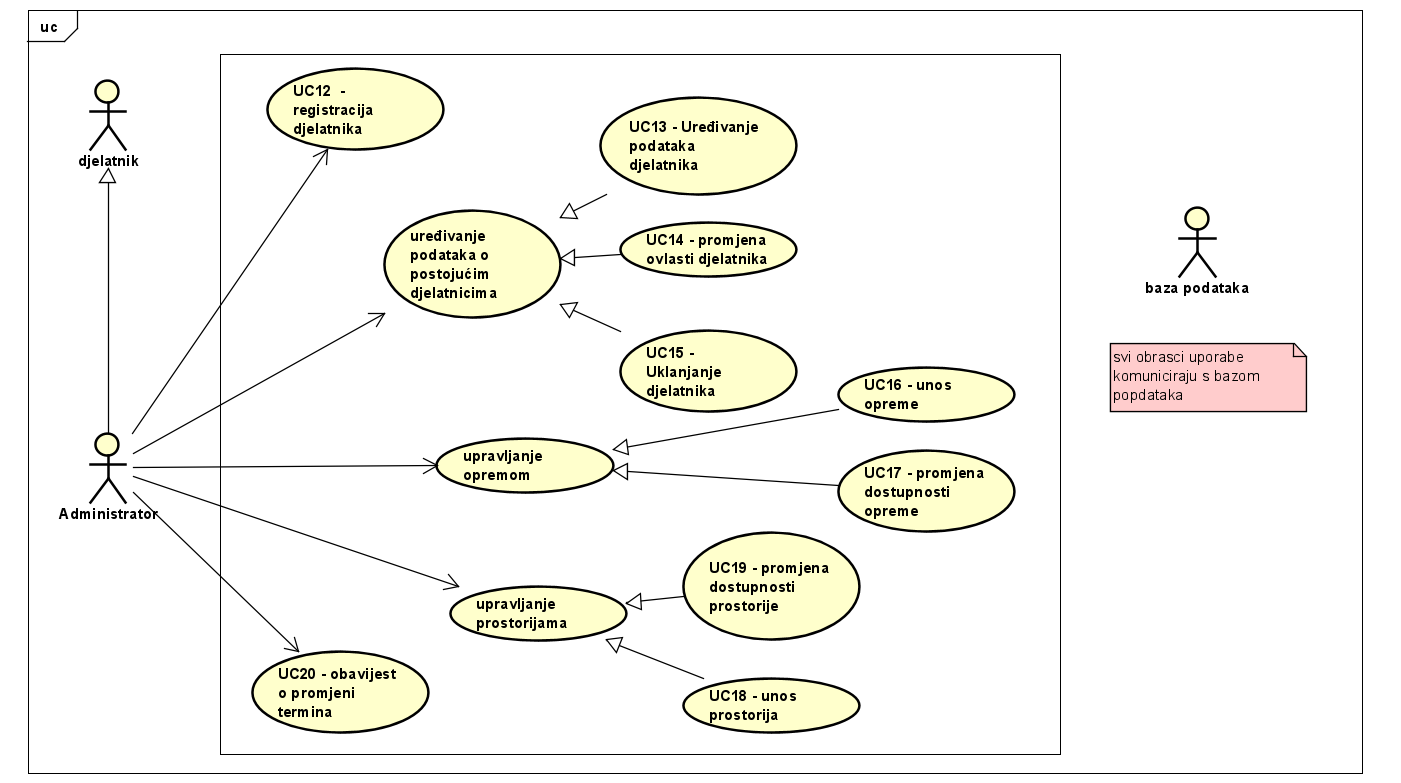
\includegraphics[scale=0.45]{slike/dijagram_obrasca_uporabe3.PNG} %veličina slike u odnosu na originalnu datoteku i pozicija slike
						\centering
						\caption{Dijagram obrasca uporabe - Administrator}
						\label{fig:dijagram_UC3}
					\end{figure}
					
				\eject		
				
			\subsection{Sekvencijski dijagrami}
				
				\textbf{\underbar{UC6 - Kreiranje terapije}}
				
				Pacijent šalje zahtjev poslužitelju za naručivanje na terapiju. Web aplikacija mu prikazuje obrazac koji mora ispuniti kako i se naručio na terapiju. Pacijent unosi potrebne podatke(ime i prezime liječnika koji ga je uputio na rehabilitaciju, vrstu terapije, opis oboljenja i zahtijevani postupak liječenja). Pacijent šalje popunjeni obrazac. Web aplikacija na temelju primljenih podataka provjerava kredibilitet liječnika u imeniku liječnika. Ovisno o rezultatu promjene web aplikacija, ako liječnik postoji u imeniku liječnika, sprema sve podatke u bazu podataka i prikazje stranicu za odabir termina. U slučaju da liječnik ne postoji u imeniku liječnika aplikacija ispisuje poruku "Liječnik ne postoji", pacijent u tom slučaju ponovno unosi to jest mijenja podatke i ponovno šalje obrazac. Pacijent može odustati od kreiranja terapije, pri čemu će mu se prikazati početna stranica.
				
				
				\begin{figure}[H]
					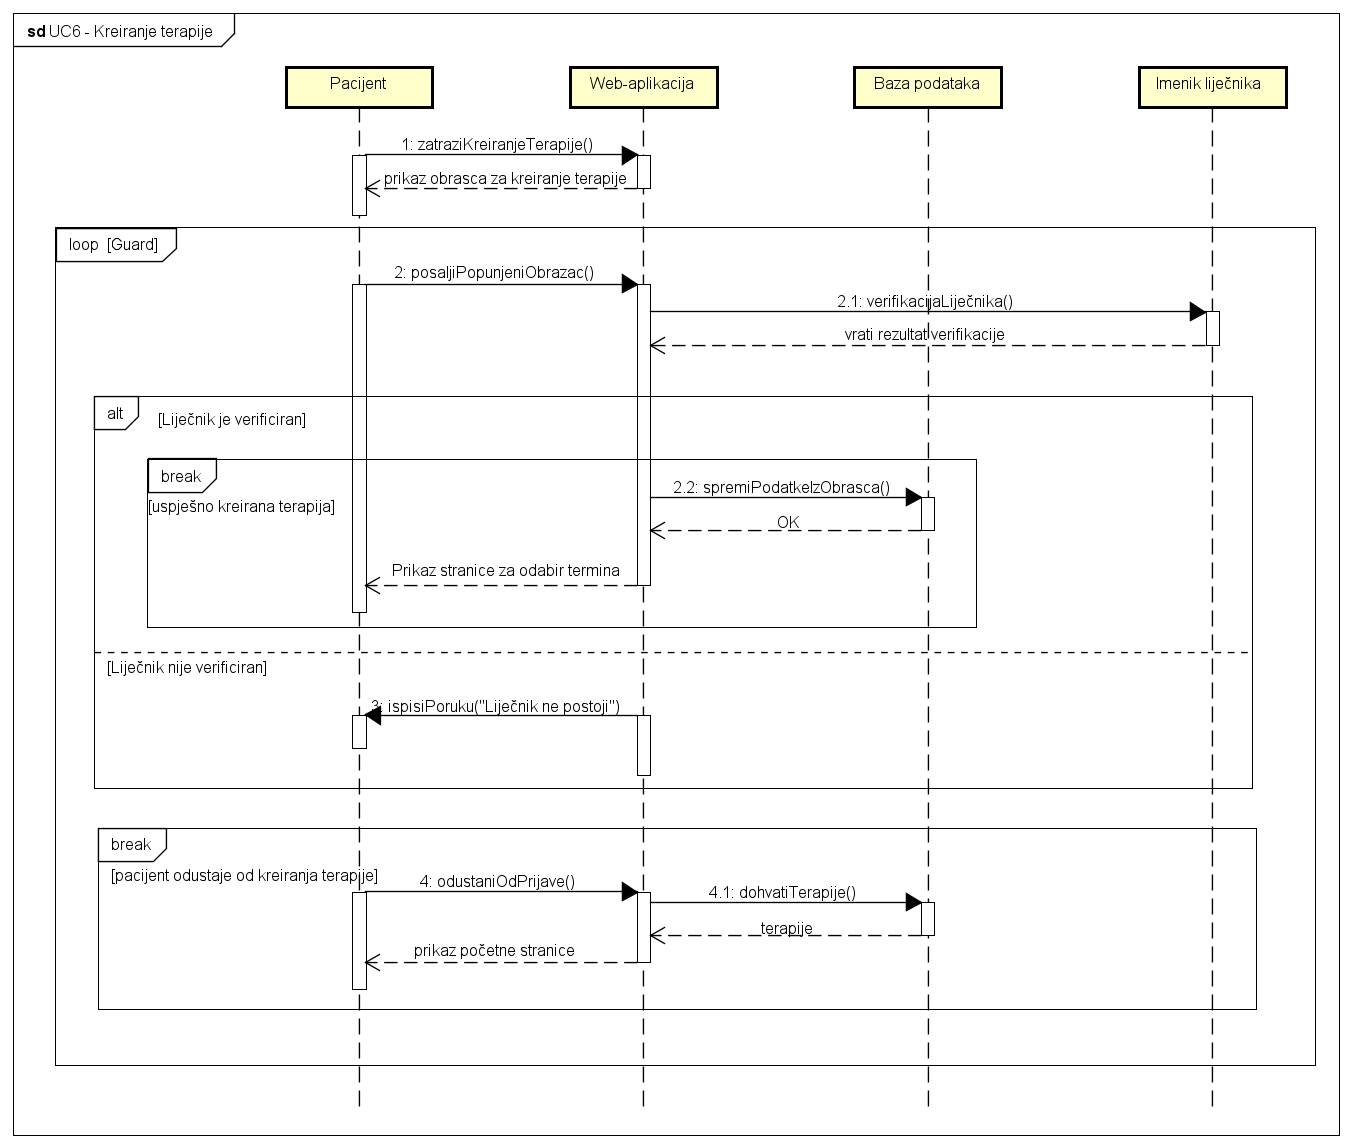
\includegraphics[scale=0.4]{slike/UC6_Kreiranje_terapije.PNG} %veličina slike u odnosu na originalnu datoteku i pozicija slike
					\centering
					\caption{Sekvencijski dijagram za UC6}
					\label{fig:sekvencijski_dijagram_1}
				\end{figure}
				
				\textbf{\underbar{UC10 - Evidencija dolaska}}
				
				Djelatnik odabire opciju evidentiraj pored termina odabranog pacijenta. Web aplikacija iz baze podataka dohvaća podatke o terapiji kojoj pripada odabrani termin, te nakon toga prikazuje obrazac za evidenciju s dohvaćenim podacima i prostorom za označavanje dolaska i unosom komentara. Djelatnik odabire status(odrađeno/ nije odrađeno) i piše komentar, nakon toga potvrđuje evidenciju i šalje popunjeni obrazac, web aplikacija potom unesene podatke sprema u bazu podataka izmjenjujući tako podatke o odabranom terminu. Nakon što su podaci uspješno uneseni web aplikacija traži od baze termine odabranog pacijenta i prikazuje stranicu s popisom termina tog pacijenta. U slučaju da je djelatnik odabrao krivi termin za evidenciju može odustati od evidentiranja, web aplikacija će dohvatiti podatke o terminima i prikazati stranicu s popisom termina odabranog pacijenta.
				
				\begin{figure}[H]
					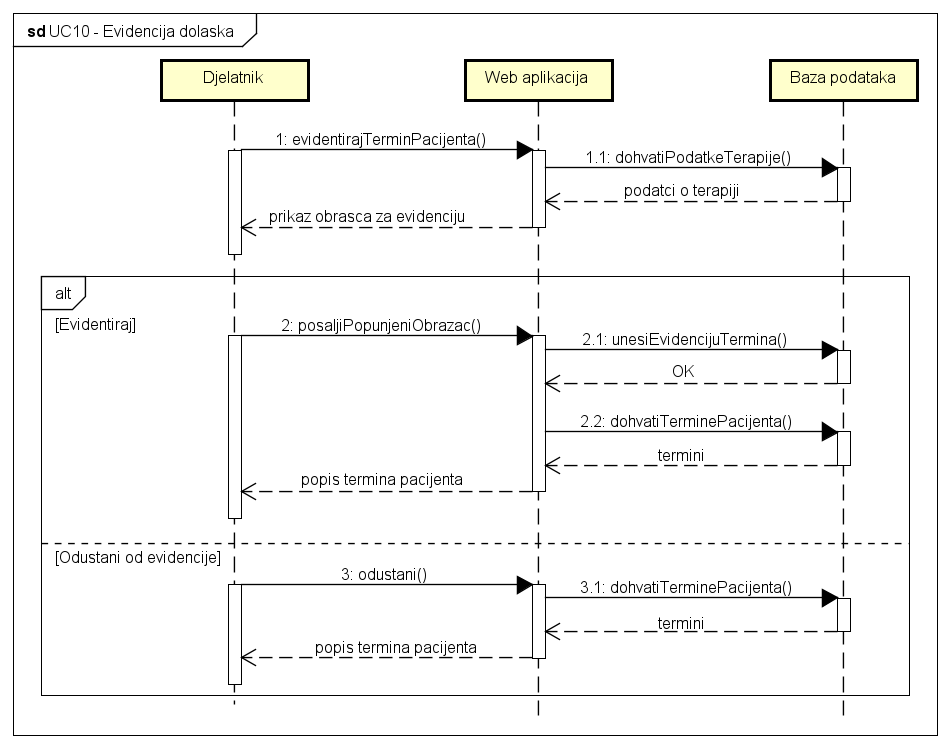
\includegraphics[scale=0.4]{slike/UC10_Evidencija_dolaska.PNG} %veličina slike u odnosu na originalnu datoteku i pozicija slike
					\centering
					\caption{Sekvencijski dijagram za UC10}
					\label{fig:sekvencijski_dijagram_2}
				\end{figure}
				
				
				\textbf{\underbar{UC19 - Obavijest o promjeni termina}}
				
				Administrator na svojoj stranici odabire opciju "Promjeni termin" te mu nakon toga web aplikacija otvara stranicu za promjenu termina. Administrator unosi pacijenta i pretražuje. Web aplikacija prima podatak i provjerava u bazi podataka ako pacijent postoji. Ako postoji web aplikacija odmah dohvaća neevidentirane termine odabranog pacijenta, te ih prikazuje administratoru. Administrator potom odabire termin koji želi promijeniti i web aplikacija mu pokazuje obrazac za dodjelu novog termina. Administrator unosi podatke o novom terminu (datum/soba/oprema) i aplikacija na temelju toga dohvaća moguće termine iz baze podataka. Administrator odabire neki od mogućih termina i opcionalno dodaje komentar. Nakon što administrator potvrdi odabrani termin web aplikacija dodaje termin u bazu podataka i šalje e-mail pacijentu s informacijama o promjeni termina, a administratoru se ponovno prikazuje stranica za promjenu termina. 
				
				U slučaju da pacijent kojeg je administrator unio ne postoji u bazi podataka aplikacija će ga obavijestiti o nepostojanju pacijenta. Administrator može ponovno unijeti pacijenta i ponoviti pretragu. 
				
				Administrator može odustati od promjene termina nakon čega mu se prikazuje početna stranica.
				
				\begin{figure}[H]
					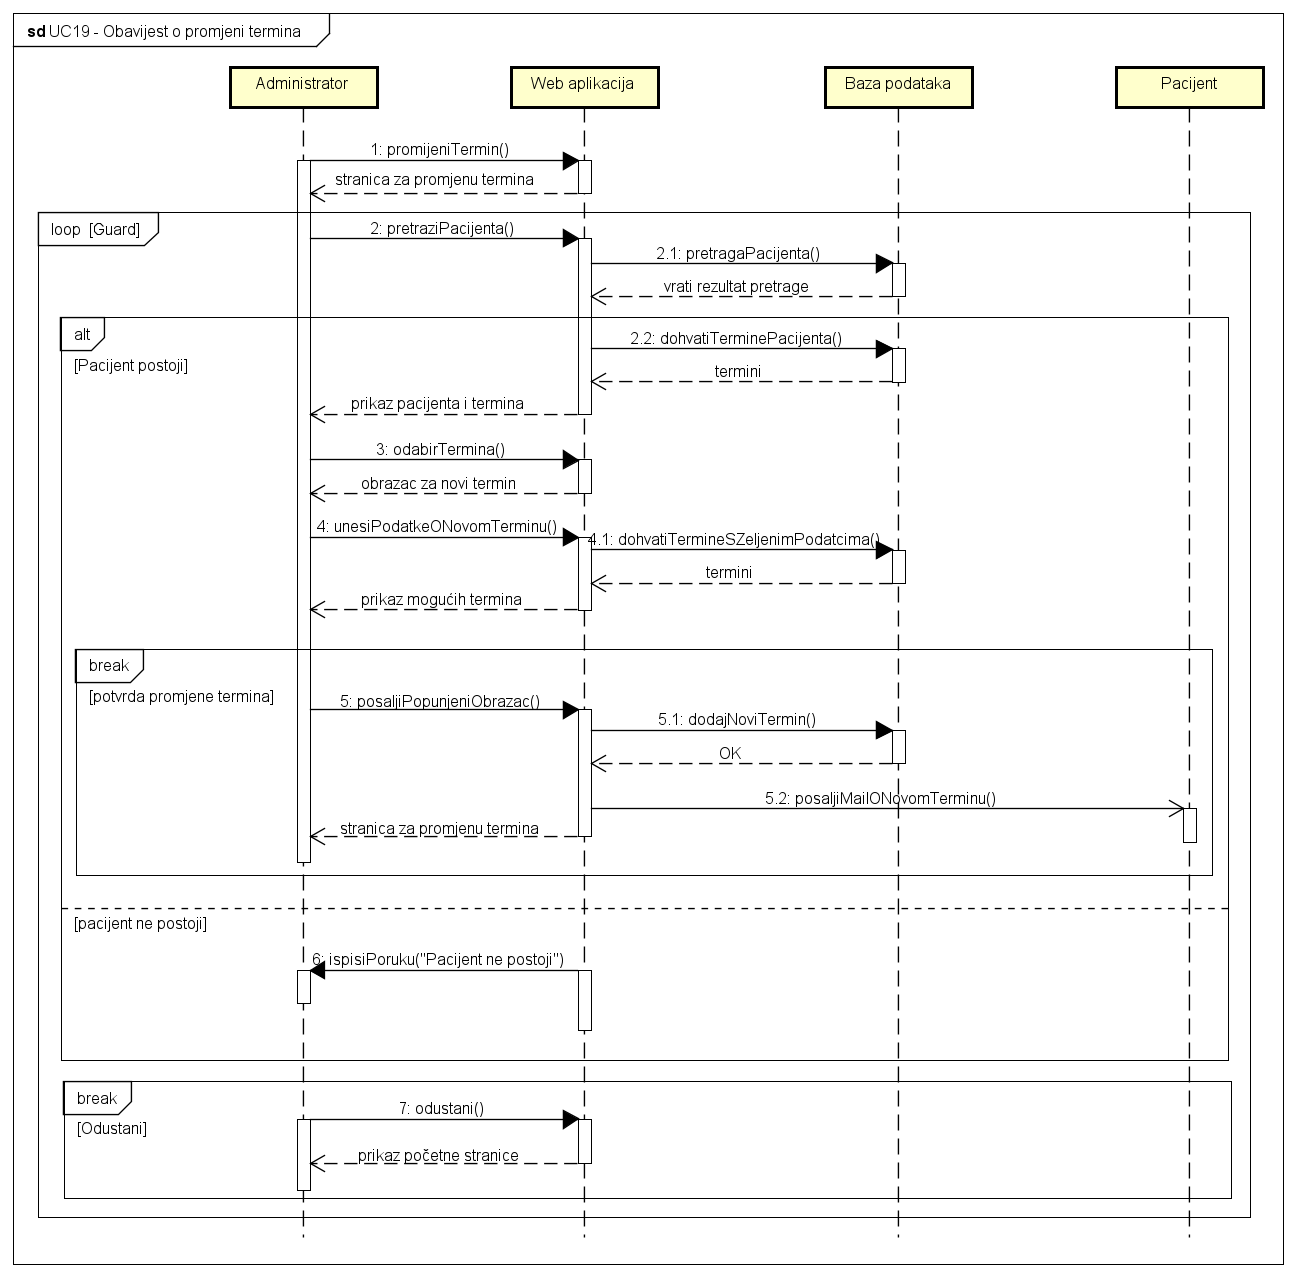
\includegraphics[scale=0.4]{slike/UC19_Obavijest_o_promjeni_termina.PNG} %veličina slike u odnosu na originalnu datoteku i pozicija slike
					\centering
					\caption{Sekvencijski dijagram za UC19}
					\label{fig:sekvencijski_dijagram_4}
				\end{figure}
				\eject
	
		\section{Ostali zahtjevi}
			 
			 \begin{packed_item}
			 	\item Sustav mora omogućiti istovremeni pristup više korisnika (100 korisnika istovremeno) uz očuvanje performansi.
			 	\item Poslužitelj mora vratiti odgovor na korisnički zahtjev unutar 5 sekundi.
			 	\item Sustav mora biti dostupan korisnicima barem 99,99\% vremena unutar jedne godine.
			 	\item Lozinka prije spremanja u bazu podataka mora biti kriptirana.
			 	\item Veza s bazom podataka mora biti brza i otporna na greške.
			 	\item Mora biti omogućen pristup sustavu iz javne mreže uz određenu razinu sigurnosti (HTTPS).
			 	\item Klijentska aplikacija mora raditi u pregledniku Google Chrome.
			 	\item Neispravno korištenje korisničkog sučelja ne smije narušiti funkcionalnost aplikacije.
			 	\item Korisničko sučelje mora podržavati hrvatski jezik.
			 	\item Korisničko sučelje mora biti jednostavno za upotrebu (intuitivno).
			 \end{packed_item}
			 
			 
			 
	
	\chapter{Arhitektura i dizajn sustava}		
	
	Sustav se može podijeliti na podsustave:
		\begin{packed_item}
			
			\item  Klijent
			\item  Poslužitelj
			\item  Baza podataka
			
		\end{packed_item}
	
		\begin{figure}[H]
			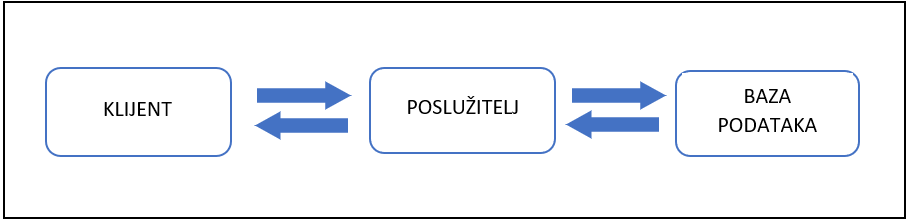
\includegraphics[width=\textwidth]{slike/Organizacija_sustava.PNG} %veličina u odnosu na širinu linije
			\caption{Organizacija sustava}
			\label{fig:organizacija_sustava1} %label mora biti drugaciji za svaku sliku
		\end{figure}
		
 
\underbar{Klijent} je web preglednik pomoću kojeg korisnici pristupaju našoj web aplikaciji. Često korišteni web preglednici su: Google Chrome, Apple Safari, Mozilla Firefox. Kada korisnik pristupa web aplikaciji, web preglednik šalje HTTP (\textit{engl. Hypertext Transfer Protocol}) zahtjeve za preuzimanje statičkih datoteka web poslužitelju. Statičke datoteke mogu biti HTML, CSS i JavaScript (React.js) datoteke. Nakon preuzimanja datoteka, preglednik ih koristi za izgradnju i prikaz korisničkog sučelja te izvršavanje funkcija unutar aplikacije. 

\underbar{Poslužitelj} je Python aplikacija pisana unutar web mikrookvira Flask. On služi kao posrednik između  klijenta (korisničkog sučelja) i baze podataka. U Python aplikaciji (Flask aplikaciji) definirani su RESTful API-ji (kao rute ili krajnje točke) koji omogućuju klijentima da šalju HTTP zahtjeve za određenim podacima. Prilikom obrade tih zahtjeva, Python aplikacija šalje upite bazi podataka kako bi dohvatila, promijenila ili dodala željene podatke.

Kada \underbar{baza podataka} zaprimi upite od poslužitelja, ona ih izvršava i vraća rezultate poslužitelju. Vraćeni rezultati mogu biti u obliku potvrde o izvršenom upitu ili u obliku podataka koje je poslužitelj zatražio od baze podataka. Baza podataka ostaje pasivna sve dok ne zaprimi nove upite od poslužitelja.

Aplikacija je organizirana po MVC (\textit{engl. Model-View-Controller, hrv. Model-Pogled-Nadglednik}) obrascu.  

Općenito, \textit{Model} definira podatke, njihovu strukturu i operacije koje se mogu izvršavati nad tim podacima. \textit{Pogled} predstavlja prikaz podataka korisniku (npr. korisničko sučelje).
\textit{Nadglednik} predstavlja posrednike između Modela i Pogleda. Oni obrađuju zahtjeve korisnika, vrše operacije nad Modelom i ažuriraju Pogled. Organizacija po ovom obrascu olakšava proširivanje i održavanje aplikacije.

Naša aplikacija ne sadrži doslovno sve tri navedene komponente. Ovdje Python objedinjuje Model i dio logike Nadglednika. Komponente u React-u odgovaraju Pogledu te je i ovdje sadržan dio logike Nadglednika.

				
		\section{Baza podataka}

Za rješavanje projektnog zadatka odabrana je relacijska baza podataka. Implementirali smo je korištenjem sustava PostgreSQL. To je besplatan sustav za upravljanje bazom podataka otvorenog koda. Objekti relacijske baze podataka su relacije. Neformalno, i u PostgreSQL-u, to su dvodimenzionalne imenovane tablice gdje imenovani stupac predstavlja atribut, a redak zapis relacije. Izbor ovakve baze podataka omogućio nam je lakše strukturiranje podatka i definiranje veza između njih, normalizaciju, skalabilnost te sigurnost kod pohrane i dohvata podataka. 
Zbog potreba naše aplikacije, baza podataka sadrži entitete:

        \begin{packed_item}
		\item 	\textnormal{Korisnik}
		\item 	\textnormal{Djelatnik}
        \item 	\textnormal{Pacijent}
        \item 	\textnormal{Terapija}
        \item 	\textnormal{VrstaTerapije}	
        \item 	\textnormal{Termin}			
        \item 	\textnormal{Status}		
        \item 	\textnormal{Soba}	
        \item 	\textnormal{Uredaj}
        \item 	\textnormal{VrstaUredaja}
        \item    SobaZa
                   				
	 \end{packed_item}

		
			\subsection{Opis tablica}
			
\textbf{Korisnik:}

Entitet Korisnik sadrži sve bitne informacije o korisniku aplikacije. Entitet sadrži atribute: idKorisnika, ime, prezime, datumRodenja, telefon, email, lozinka, potvrden, potvrdenNa. Atribut idKorisnika je primarni ključ. Atributi email i telefon su alternativni ključevi. Korisnik može biti ili djelatnik zdravstvene ustanove ili pacijent koji se želi naručiti na terapiju u zdravstvenoj ustanovi. 

				
				
				\begin{longtblr}[
					label=none,
					entry=none
					]{
						width = \textwidth,
						colspec={|X[6,l]|X[7, l]|X[20, l]|}, 
						rowhead = 1,
					} %definicija širine tablice, širine stupaca, poravnanje i broja redaka naslova tablice
					\hline \SetCell[c=3]{c}{\textbf{Korisnik}}	 \\ \hline[3pt]
					\SetCell{LightGreen}idKorisnika & INT & jedinstveni identifikator korisnika 	\\ \hline
					ime & VARCHAR(50) & ime korisnika	\\ \hline 
                     prezime & VARCHAR(50) & prezime korisnika	\\ \hline
                     datumRodenja & DATE & datum rođenja korisnika	\\ \hline  
                     telefon & VARCHAR(20) & broj mobilnog telefona korisnika	\\ \hline 
					email & VARCHAR(100) & e-mail adresa korisnika   \\ \hline 
					lozinka & VARCHAR(100) & hash lozinke za prijavu u aplikaciju	\\ \hline
					potvrden & BOOLEAN & status potvrde e-maila korisnika (e-mail je ili nije potvrđen) 	\\ \hline
					potvrdenNa & TIMESTAMP & datum i vrijeme potvrde e-maila korisnika	\\ \hline
					 
				\end{longtblr}

\textbf{Djelatnik:}

Entitet Djelatnik je ekskluzivna specijalizacija entiteta Korisnik. Entitet sadrži atribute: idKorisnika, jeAktivan, jeAdmin, OIB. Djelatnik je povezan s Korisnikom preko atributa idKorisnika. Atribut OIB je alternativni ključ.

				\begin{longtblr}[
					label=none,
					entry=none
					]{
						width = \textwidth,
						colspec={|X[6,l]|X[7, l]|X[20, l]|}, 
						rowhead = 1,
					} %definicija širine tablice, širine stupaca, poravnanje i broja redaka naslova tablice
					\hline \SetCell[c=3]{c}{\textbf{Djelatnik}}	 \\ \hline[3pt]
					\SetCell{LightBlue}idKorisnika & INT & jedinstveni identifikator korisnika (korisnik.idKorisnika) 	\\ \hline
					OIB & CHAR(11) & osobni identifikacijski broj pacijenta	\\ \hline
					jeAktivan & BOOLEAN & označava radni odnos liječnika i zdravstvene ustanove (radi = true, ne radi = false)	\\ \hline 
					jeAdmin & BOOLEAN & označava je li djelatnik administrator (true = je, false = nije)	\\ \hline
					
					 
				\end{longtblr}

\textbf{Pacijent:}

Entitet Pacijent je ekskluzivna specijalizacija entiteta Korisnik. Entitet sadrži atribute: idKorisnika, MBO. Pacijent je povezan s Korisnikom preko atributa idKorisnika (korisnik.idKorisika). Atribut MBO je alternativni ključ.

				\begin{longtblr}[
					label=none,
					entry=none
					]{
						width = \textwidth,
						colspec={|X[6,l]|X[7, l]|X[20, l]|}, 
						rowhead = 1,
					} %definicija širine tablice, širine stupaca, poravnanje i broja redaka naslova tablice
					\hline \SetCell[c=3]{c}{\textbf{Pacijent}}	 \\ \hline[3pt]
					\SetCell{LightBlue}idKorisnika & INT & jedinstveni identifikator korisnika (korisnik.idKorisnika)	\\ \hline
					MBO & CHAR(9) & matični broj osiguranika (pacijenta)	\\ \hline 

					 
				\end{longtblr}

\textbf{Terapija:}

Entitet Terapija sadrži sve bitne informacije o terapiji na koju je pacijent naručen. Entitet sadrži atribute: idTerapije, idLijecnika, opisOboljenja, zahtPostLijec, datumPoc, datumZavrs, idPacijenta, idVrste. Atributi zahtPostLijec, datumPoc, datumZavrs i idVrste su opcionalni. Entitet Terapija je povezan binarnom N:1 vezom s entitetom Pacijentom preko atributa idPacijenta. Entitet Terapija je povezan binarnom N:1 vezom s entitetom VrstaTerapije preko atributa idVrste.

				\begin{longtblr}[
					label=none,
					entry=none
					]{
						width = \textwidth,
						colspec={|X[6,l]|X[7, l]|X[20, l]|}, 
						rowhead = 1,
					} %definicija širine tablice, širine stupaca, poravnanje i broja redaka naslova tablice
					\hline \SetCell[c=3]{c}{\textbf{Terapija}}	 \\ \hline[3pt]
					\SetCell{LightGreen}idTerapije & INT & jedinstveni identifikator terapije	\\ \hline
					idLijecnika & INT & jedinstveni identifikator liječnika	\\ \hline 
                    opisOboljenja & VARCHAR(300) & opis oboljenja pacijenta	\\ \hline
                    zahtPostLijec & VARCHAR(300) & zahtjev za postupkom liječenja (terapijom)	\\ \hline  
                    datumPoc & DATETIME & datum početka terapije	\\ \hline 
					 datumZavrs & DATETIME & datum završetka terapije   \\ \hline 
					 \SetCell{LightBlue}idPacijenta & INT & jedinstveni identifikator pacijenta (pacijent.idKorisnika)	\\ \hline 
					 \SetCell{LightBlue}idVrste & INT & jedinstveni identifikator vrste uređaja (vrstaTerapije.idVrste) \\ \hline
					 
				\end{longtblr}

\textbf{VrstaTerapije:}

Entitet VrstaTerapije sadrži sve bitne informacije o vrsti terapije na koju je pacijent naručen. Entitet sadrži atribute: idVrste, imeVrste, opisVrste. Atribut idVrste je primarni ključ. Atribut opisVrste je opcionalan. Entitet VrstaTerapije povezan je binarnom N:N vezom s entitetom Soba.

\begin{longtblr}[
					label=none,
					entry=none
					]{
						width = \textwidth,
						colspec={|X[6,l]|X[7, l]|X[20, l]|}, 
						rowhead = 1,
					} %definicija širine tablice, širine stupaca, poravnanje i broja redaka naslova tablice
					\hline \SetCell[c=3]{c}{\textbf{VrstaTerapije}}	 \\ \hline[3pt]
					\SetCell{LightGreen}idVrste & INT & jedinstveni identifikator vrste terapije	\\ \hline
					imeVrste & VARCHAR(50) & naziv vrste terapije	\\ \hline 
                     opisVrste & VARCHAR(300) & opis vrste terapije	\\ \hline
					 
				\end{longtblr}

\textbf{Termin:}

Entitet Termin sadrži sve bitne informacije o terminu terapije na koji je pacijent naručen. Entitet Termin ne postoji bez entiteta vlasnika, entiteta Terapija (Termin je egzistencijalno slab entitet). Atribut idTermina je primarni ključ, dok su idTerapije, brSobe, idStatus i idDjelatnika strani ključevi. Atributi do, komentar i idDjelatnika su opcionalni. Entitet Termin povezan je binarnom N:1 vezom s entitetom Terapija preko atributa idTerapije. Entitet Termin povezan je binarnom N:1 vezom s entitetom Soba preko atributa brSobe. Entitet Termin povezan je binarnom N:1 vezom s entitetom Status preko atributa idStatus. Entitet Termin povezan je binarnom N:0..1 vezom s entitetom Djelatnik preko atributa idKorisnika.
\textit{Napomena: Primarni ključ entiteta Termin je kompozitni ključ (idTermina, idTerapije).}

\begin{longtblr}[
					label=none,
					entry=none
					]{
						width = \textwidth,
						colspec={|X[6,l]|X[7, l]|X[20, l]|}, 
						rowhead = 1,
					} %definicija širine tablice, širine stupaca, poravnanje i broja redaka naslova tablice
					\hline \SetCell[c=3]{c}{\textbf{Termin}}	 \\ \hline[3pt]
					\SetCell{LightGreen}idTermina & INT & jedinstveni identifikator termina terapije \\ \hline
					\SetCell{LightBlue}idTerapije & INT & jedinstveni identifikator terapije (terapija.idTerapije)	\\ \hline 
					\SetCell{LightBlue}idDjelatnika & INT & jedinstveni identifikator djelatnika (djelatnik.idKorisnika)	\\ \hline
                     od & TIMESTAMP & datum i vrijeme početka termina	\\ \hline
					 do & TIMESTAMP & datum i vrijeme završetka termina      \\ \hline
                     komentar & VARCHAR(300) & komentar liječnika o napretku terapije \\ \hline
                     \SetCell{LightBlue}brSobe & VARCHAR(10) & jedinstveni identifikator sobe (soba.brSobe)	\\ \hline
                     \SetCell{LightBlue}idStatus & INT & jedinstveni identifikator statusa (status.idStatus)	\\ \hline
                                          
				\end{longtblr}

\textbf{Soba:}

Entitet Soba sadrži sve bitne informacije o sobi u kojoj se provodi neka terapija. Entitet sadrži atribute: brSobe, kapacitet, uUporabi. Atribut brSobe je primarni ključ. Entitet Soba povezan je binarnom N:N vezom s entitetom VrstaTerapije.

\begin{longtblr}[
					label=none,
					entry=none
					]{
						width = \textwidth,
						colspec={|X[6,l]|X[7, l]|X[20, l]|}, 
						rowhead = 1,
					} %definicija širine tablice, širine stupaca, poravnanje i broja redaka naslova tablice
					\hline \SetCell[c=3]{c}{\textbf{Soba}}	 \\ \hline[3pt]
					\SetCell{LightGreen}brSobe & VARCHAR(10) & jedinstveni identifikator sobe \\ \hline
                     kapacitet & INT & kapacitet sobe, broj pacijenata koji istovremeno mogu biti na terapiji u nekoj sobi	\\ \hline
                     uUporabi & BOOLEAN & označava je li soba popunjena (true = popunjena, false = nije popunjena)	\\ \hline
				\end{longtblr}
				
\textbf{SobaZa:}

Entitet SobaZa sadrži sve bitne informacije o sobi u kojoj se odvija točno određena vrsta terapije. Entitet SobaZa sadrži atribute brSobe i idVrste. Atributi brSobe i idVrste su strani ključevi. 

				\begin{longtblr}[
					label=none,
					entry=none
					]{
						width = \textwidth,
						colspec={|X[6,l]|X[7, l]|X[20, l]|}, 
						rowhead = 1,
					} %definicija širine tablice, širine stupaca, poravnanje i broja redaka naslova tablice
					\hline \SetCell[c=3]{c}{\textbf{SobaZa}}	 \\ \hline[3pt]
					\SetCell{LightBlue}brSobe & INT & jedinstveni identifikator sobe (soba.brSobe)	\\ \hline
					\SetCell{LightBlue}idVrste & INT & jedinstveni identifikator vrste terapije (vrstaTerapije.idVrste)	\\ \hline 

					 
				\end{longtblr}

\textbf{Uredaj:}

Entitet Uredaj sadrži sve bitne informacije o uređaju. Entitet sadrži atribute: idUredaja, brSobe, idVrste. Atribut idUredaja je primarni ključ, dok su atributi brSobe i idVrste strani ključevi. Atribut brSobe je opcionalan. Entitet Uredaj povezan je binarnom N:0..1 vezom s entitetom Soba preko atributa brSobe. Entitet Uredaj povezan je binarnom N:1 vezom s entitetom VrstaUredaja preko atributa idVrste.

\begin{longtblr}[
					label=none,
					entry=none
					]{
						width = \textwidth,
						colspec={|X[6,l]|X[7, l]|X[20, l]|}, 
						rowhead = 1,
					} %definicija širine tablice, širine stupaca, poravnanje i broja redaka naslova tablice
					\hline \SetCell[c=3]{c}{\textbf{Uredaj}}	 \\ \hline[3pt]
					\SetCell{LightGreen}idUredaja & INT & jedinstveni identifikator uređaja \\ \hline
                    \SetCell{LightBlue}brSobe & VARCHAR(10) & jedinstveni identifikator sobe (soba.brSobe) \\ \hline
                     \SetCell{LightBlue}idVrste & INT & jedinstveni identifikator vrste uređaja (vrstaUredaja.idVrste)\\ \hline
				\end{longtblr}

\textbf{VrstaUredaja:}

Entitet VrstaUredaja sadrži sve bitne informacije o vrsti uređaja. Entitet sadrži atribute: idVrste, imeVrste, opisVrste. Atribut idVrste je primarni ključ. Atribut opisVrste je opcionalan.

\begin{longtblr}[
					label=none,
					entry=none
					]{
						width = \textwidth,
						colspec={|X[6,l]|X[7, l]|X[20, l]|}, 
						rowhead = 1,
					} %definicija širine tablice, širine stupaca, poravnanje i broja redaka naslova tablice
					\hline \SetCell[c=3]{c}{\textbf{VrstaUredaja}}	 \\ \hline[3pt]
					\SetCell{LightGreen}idVrste & INT & jedinstveni identifikator vrste uređaja \\ \hline
                     imeVrste & VARCHAR(50) & naziv vrste uređaja \\ \hline
                     opisVrste & VARCHAR(300) & opis vrste uređaja \\ \hline
				\end{longtblr}


\textbf{Status:}

Entitet Status sadrži sve bitne informacije o statusu termina terapije koji je dodijeljen pacijentu. Entitet sadrži atribute: idStatus, imeStatus. Atribut idStatus je primarni ključ.

\begin{longtblr}[
					label=none,
					entry=none
					]{
						width = \textwidth,
						colspec={|X[6,l]|X[7, l]|X[20, l]|}, 
						rowhead = 1,
					} %definicija širine tablice, širine stupaca, poravnanje i broja redaka naslova tablice
					\hline \SetCell[c=3]{c}{\textbf{Status}}	 \\ \hline[3pt]
					\SetCell{LightGreen}idStatus & INT & jedinstveni identifikator uređaja \\ \hline
                     imeStatus & VARCHAR(50) & naziv statusa (npr. u tijeku, završen) \\ \hline
     
				\end{longtblr}	
				
			
			\subsection{Dijagram baze podataka}
		\begin{figure}[H]
			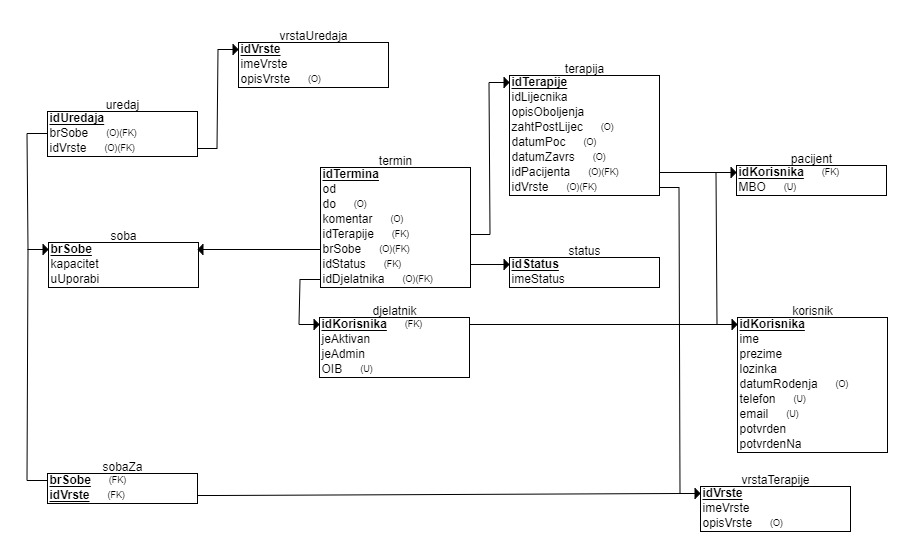
\includegraphics[width=\textwidth]{slike/Relacijska_shema_baze_podataka.JPG} %veličina u odnosu na širinu linije
			\caption{Relacijska shema baze podataka}
			\label{fig:relacijska_shema1} %label mora biti drugaciji za svaku sliku
		\end{figure}
		
		\begin{figure}[H]
			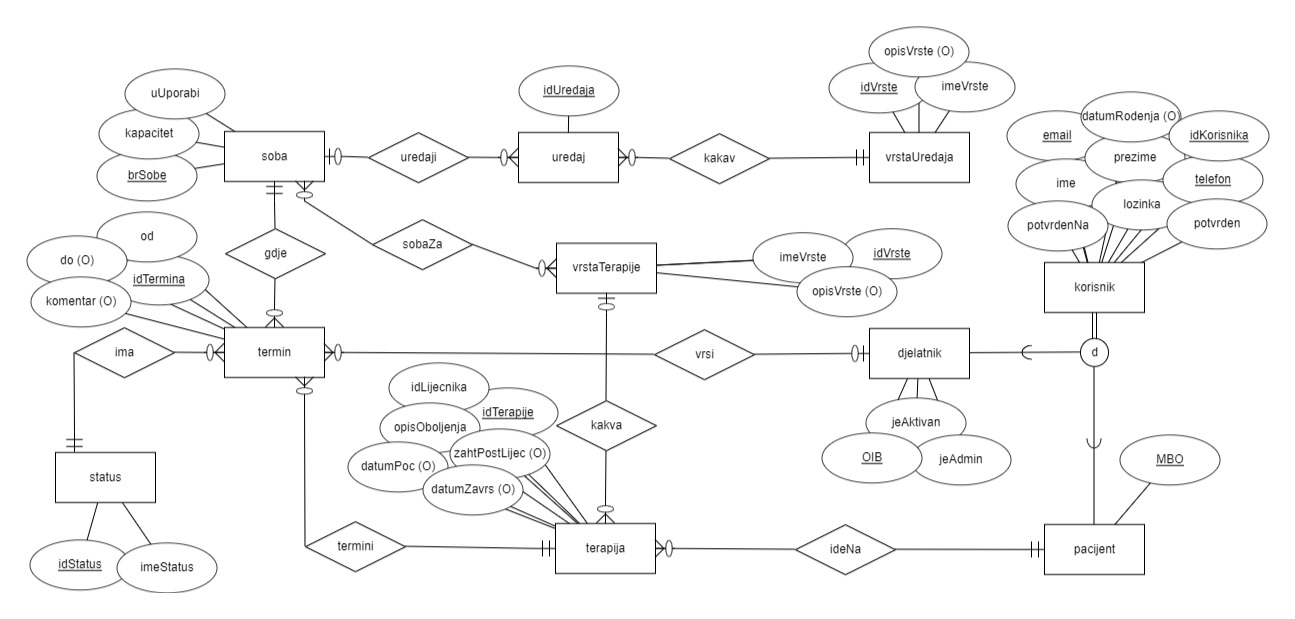
\includegraphics[width=\textwidth]{slike/ER_model_baze_podataka.JPG} %veličina u odnosu na širinu linije
			\caption{ER model baze podataka}
			\label{fig:er_model} %label mora biti drugaciji za svaku sliku
		\end{figure}
			
		\section{Dijagram razreda}
		
			Dijagrami razreda rađeni su po uzoru na MVC obrazac po kojem je naša aplikacija organizirana. Podijeljeni su u 3 dijela: Nadglednik(\textit{Controller}) (\ref{fig:dijagram_razreda_1}), DTO (\ref{fig:dijagram_razreda_2}) i Model (\ref{fig:dijagram_razreda_3}).
			
			Nadglednik (\textit{Controller}) obrađuje zahtjeve korisnika i preko DTO-a(\textit{Data transfer object}) vrši operacije nad Modelom. Zamišljeno je da funkcije implementirane u Nadgledniku vraćaju html status kod. \textit{KorisnikController} ima funkcije za dohvaćanje, stvaranje i izmjenjivanje korisnika(pacijenta i djelatnika). \textit{TerminController} ima funkcije za dohvaćanje, izmjenjivanje i dodavanje termina i statusa koji je povezan za njega. \textit{VerifikacijaController} ima funkcije za verifikaciju i slanje e-maila, promjenu lozinke, prijavu i registraciju korisnika. \textit{InventarController} sadrži funkcije za dodavanje, brisanje i izmjenjivanje inventara/uređaja. \textit{SobaController} ima funkcije za dohvaćanje, uređivanje i stvaranje soba. \textit{TerapijaController} ima funkcije za stvaranje, dohvaćanje i uređivanje prostorija.
			\begin{figure}[H]
				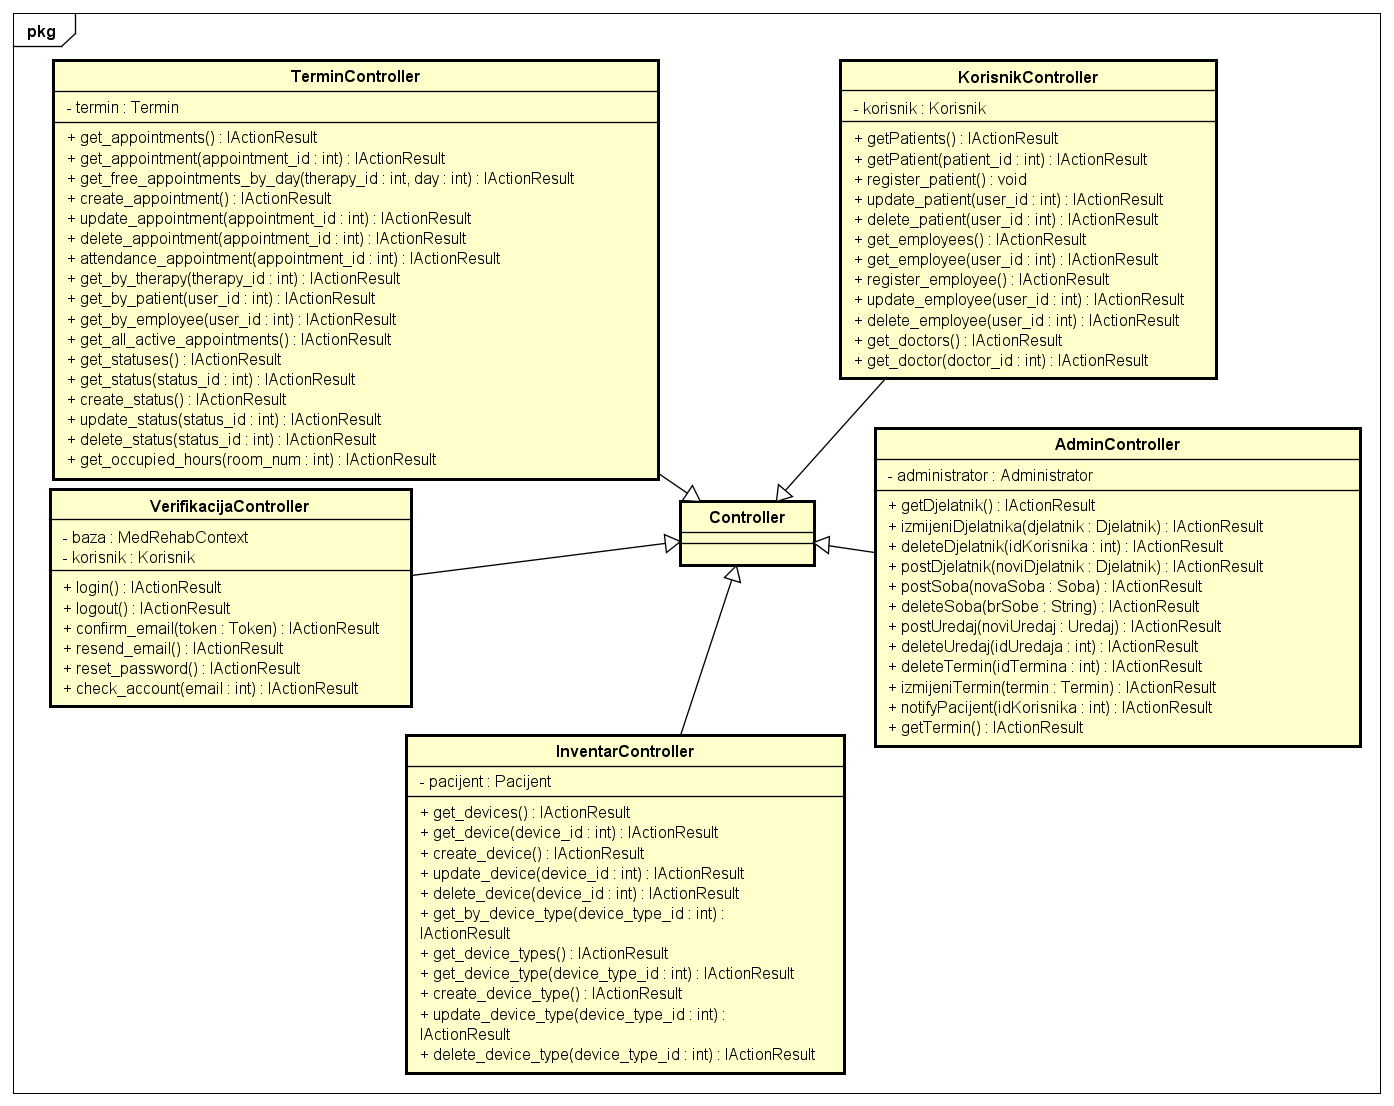
\includegraphics[scale=0.41]{slike/Dijagram_razreda_1.PNG} %veličina slike u odnosu na originalnu datoteku i pozicija slike
				\centering
				\caption{Dijagram razreda za dio Controller}
				\label{fig:dijagram_razreda_1}
			\end{figure}
			
			Dio s DTO-om sadrži jednostavne klase i služi isključivo za prenošenje podataka kako bi Nadglednik mogao vršiti operacije nad Modelom. Sadrži klase slične dijagramu razreda za dio Model uz nekoliko iznimaka. \textit{TerapijaSTerminima} sadrži atribute terapije s listom termina koji su vezanu uz pojedinu terapiju. \textit{ZahtjevPacijentaDTO} sadrži atribute Terapije i Termina koji su potrebni da bi Pacijent mogao napraviti Zahtjev.
			
			\begin{figure}[H]
				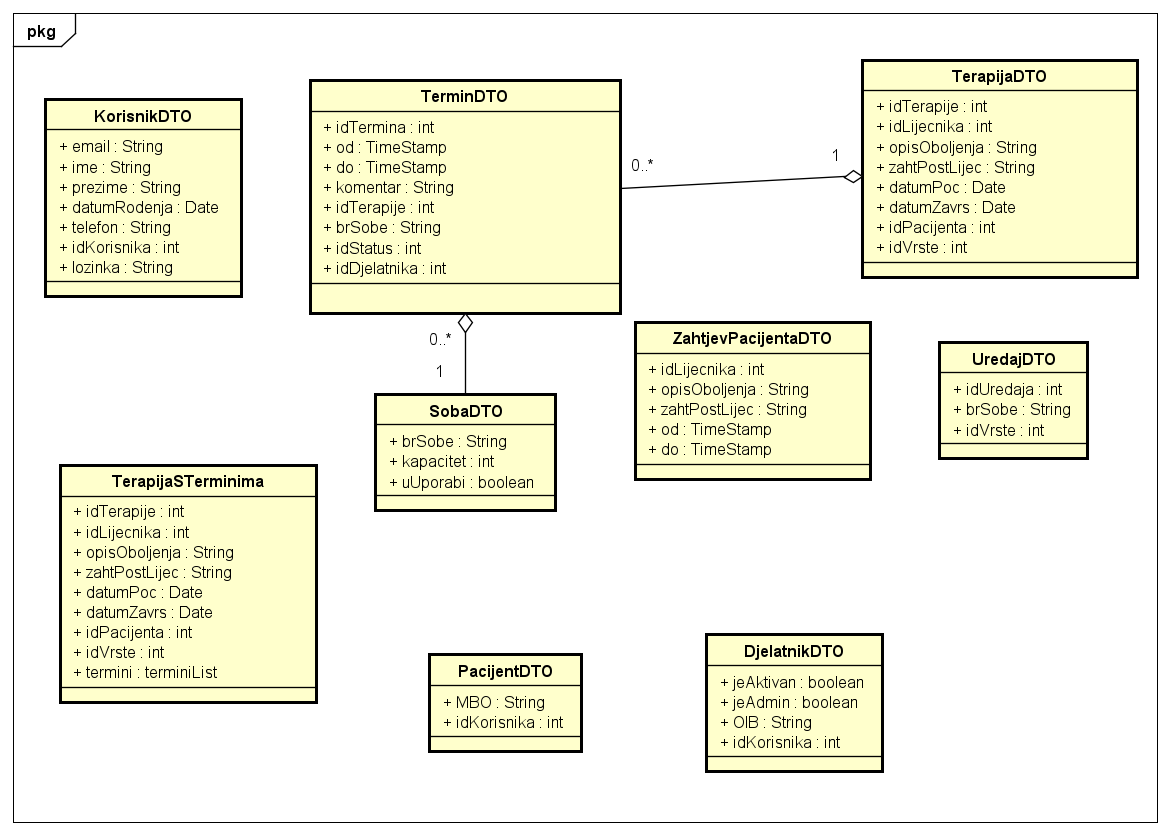
\includegraphics[scale=0.3]{slike/Dijagram_razreda_2.PNG} %veličina slike u odnosu na originalnu datoteku i pozicija slike
				\centering
				\caption{Dijagram razreda za dio DTO}
				\label{fig:dijagram_razreda_2}
			\end{figure}
			
			Model sadrži atribute i metode koje su potrebne radi komunikacije s bazom podataka. Razred \textit{Korisnik} predstavlja korisnika koji, ako je neprijavljen, ima funkciju registracije, a ako je prijavljen, ima funkciju prikaza i promjene osobnih podataka. \textit{Administrator} predstavlja korisnika koji upravlja djelatnicima, sobama i uređajima i obavještava pacijenta ukoliko je potrebno. \textit{Djelatnik} je liječnik koji ima opciju pregleda pacijenta, njegovih termina i evidencije njegovih termina, evidencije pacijenta i prihvaćanje ili odbijanje zahtjeva za terminom. Razred \textit{Pacijent} je pacijent koji može pregledati predane zahtjeve i termine, filtrirati termine, pregledati nalaze terapije i naručiti novu terapiju. Prisutne su i klase Terapija, vrstaTerapije, Termin, Status, Soba, Uredaj i VrstaUredaja koje za sada nemaju predviđene nikakve funkcije. Svaki razred sadrži atribute bitne za taj razred.
			
			\begin{figure}[H]
				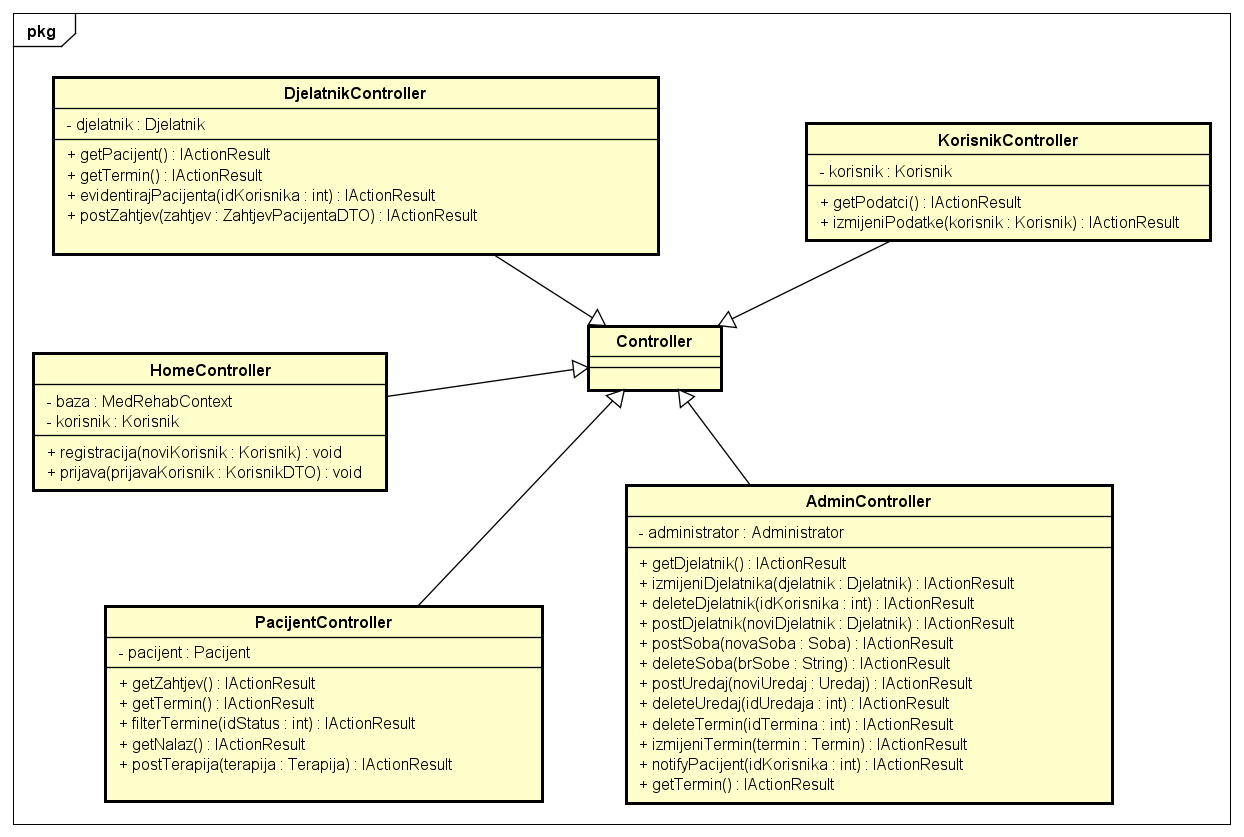
\includegraphics[scale=0.45]{slike/Dijagram_razreda_3.PNG} %veličina slike u odnosu na originalnu datoteku i pozicija slike
				\centering
				\caption{Dijagram razreda za dio Model}
				\label{fig:dijagram_razreda_3}
			\end{figure}
			
			
			
			
			\eject
		
		\section{Dijagram stanja}
			
			
			Dijagram stanja (\ref{fig:dijagram_stanja1}) prikazuje stanja i prijelaze između stanja u kojima se nalazi korisničko sučelje kada korisnik - pacijent koristi aplikaciju. Stanje u dijagramu predstavlja ekran (\textit{engl. screen}) u aplikaciji, a prijelaz predstavlja radnju korisnika kada koristi aplikaciju (klik na gumb ili ikonu).
			Kada se korisnik registrira i prijavi u aplikaciju, prvo mu se prikaže početni ekran. Klikom na gumb 'Moje terapije', korisniku se prikazuje ekran s listom terapija. Na ekranu s listom terapija korisnik vidi svoje terapije i pripadajuće informacije te može dodati novu terapiju klikom na gumb 'Dodaj terapiju'. Kada korisnik dodaje novu terapiju, otvara mu se ekran s obrascem u koji mora unijeti informacije o terapiji. Ako su uneseni podaci ispravni, korisnika se vraća na ekran s listom terapija u koju je dodana i nova terapija. Ako uneseni podaci nisu ispravni, korisnika se vraća na ekran s obrascem te on može ponovno unijeti podatke ili odustati od dodavanja nove terapije. Klikom na terapiju s liste terapija, korisniku se prikazuje novi ekran s informacijama o terapiji i listom termina te njihovim informacijama (dalje: ekran s listom termina). Ako terapija još uvijek traje, korisnik može poslati zahtjev za novim terminom klikom na gumb 'Dodaj termin'. Kada korisnik dodaje novi termin, prikaže mu se ekran s obrascem u koji mora unijeti podatke o terminu. Kada korisnik ispuni obrazac i klikne na gumb 'Pošalji', vraća ga se na ekran s listom termina (na listi je prikazan i novi termin). Klikom na termin s liste termina, korisniku se prikazuje ekran s detaljnim informacijama o terminu te mogućnost otkazivanja termina klikom na gumb 'Otkaži', ako je status termina 'zakazan'. U slučaju otkazivanja termina, korisnika se vraća na ekran s listom termina - otkazani termin se i dalje nalazi u listi termina, ali s promijenjenim statusom ('otkazan'). Klikom na gumb 'Korisnički račun', korisniku se prikazuje ekran s korisničkim informacijama i mogućnošću promjene broja telefona ili lozinke. Klikom na gumb 'Promijeni lozinku', korisniku se prikazuje ekran s obrascem za promjenu lozinke. Ako su podaci uneseni u obrazac ispravni, korisnik na ekranu dobiva potvrdu o uspješnoj promjeni lozinke te ga se vraća na ekran s ažuriranim korisničkim informacijama. Ako uneseni podaci nisu ispravni, korisnika se vraća na obrazac te on ima mogućnost ponovnog unosa podataka ili odustajanja od promjene podataka i vraćanja na ekran s korisničkim informacijama. Isti proces se odvija i u slučaju promjene broja telefona - klikom na gumb 'Promijeni broj telefona'. Korisnik se može odjaviti iz aplikacije klikom na gumb 'Odjavi se', bez obzira na kojem se ekranu nalazi. Također, korisnik u svakom trenutku ima mogućnost povratka na početni ekran, ekran s prikazom terapija ili ekran s korisničkim informacija klikom na odgovarajući gumb.
			
			\begin{figure}[H]
				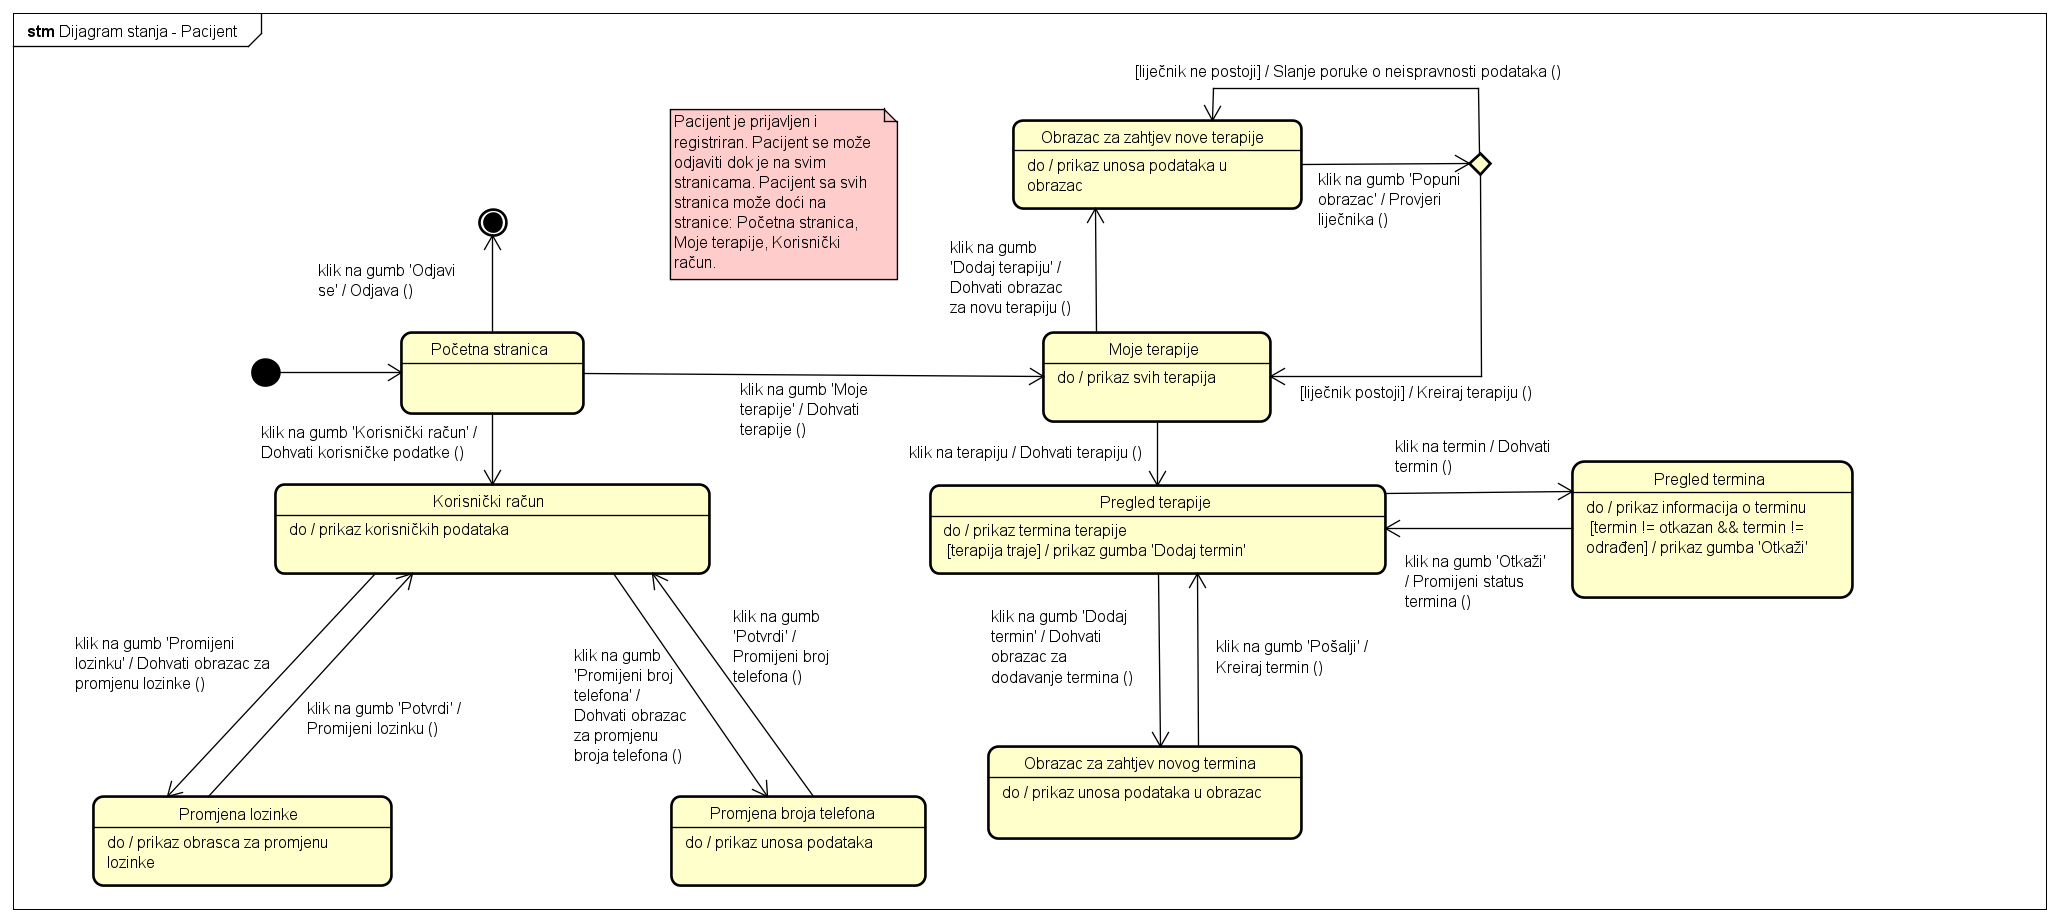
\includegraphics[scale=0.3]{slike/Dijagram stanja - Pacijent.PNG} %veličina slike u odnosu na originalnu datoteku i pozicija slike
				\centering
				\caption{Dijagram stanja}
				\label{fig:dijagram_stanja1}
			\end{figure}
			
			
			\eject 
		
		\section{Dijagram aktivnosti}
		
			

Dijagram aktivnosti - Kreiranje terapije (\ref{fig:dijagram_aktivnoti_terapija}) prikazuje proces prijave korisnika (pacijenta) na novu terapiju. Kada korisnik zatraži novu terapiju, prikazuje mu se obrazac koji popunjava s podacima o terapiji. Ako su podaci neispravni, sustav mu dojavljuje grešku i vraća ga na obrazac. Ako su podaci ispravni, nova terapija mu se prikaže na listi terapija. 

\begin{figure}[H]
				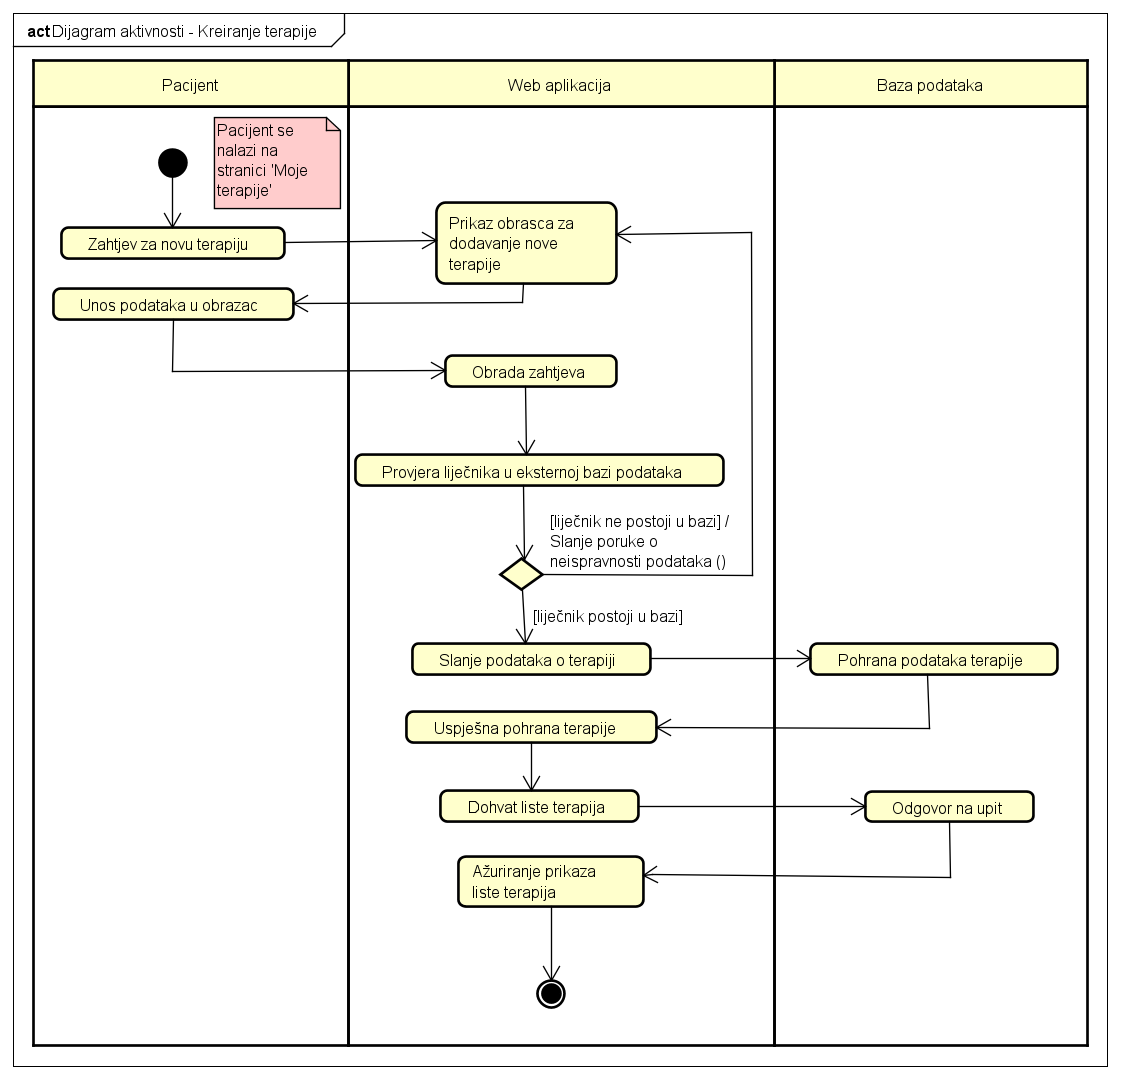
\includegraphics[scale=0.3]{slike/Dijagram_aktivnosti _Kreiranje_terapije.PNG} %veličina slike u odnosu na originalnu datoteku i pozicija slike
				\centering
				\caption{Dijagram aktivnosti za kreiranje terapije}
				\label{fig:dijagram_aktivnoti_terapija}
			\end{figure}
Dijagram aktivnosti - Dodavanje termina (\ref{fig:dijagram_aktivnosti_termin}) prikazuje proces naručivanja korisnika (pacijenta) na novi termin odabrane terapije. Kada korisnik zatraži novi termin, prikazuje mu se obrazac koji popunjava s podacima o terminu. Ako su podaci neispravni, sustav mu dojavljuje grešku i vraća ga na obrazac. Ako su podaci ispravni, novi termin se prikaže u listi termina.

\begin{figure}[H]
				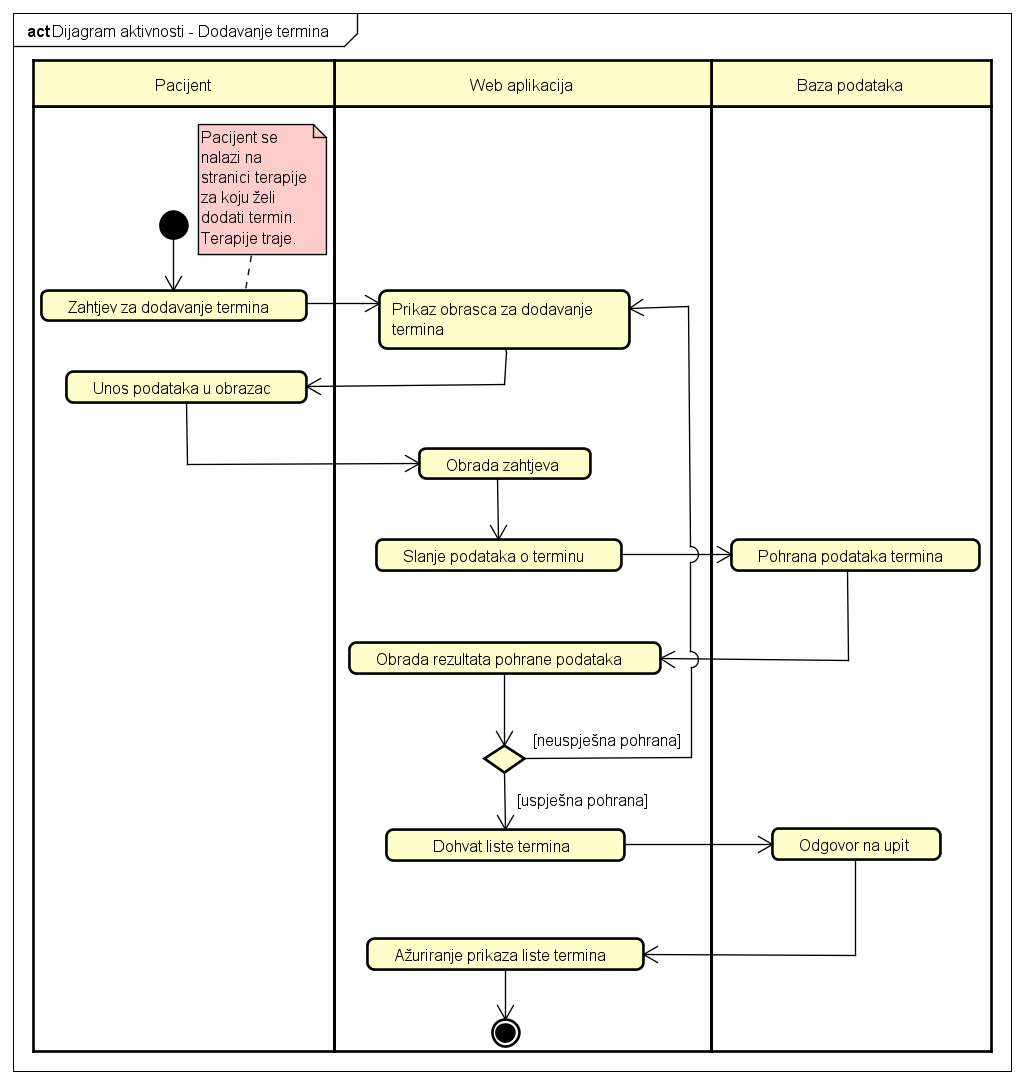
\includegraphics[scale=0.3]{slike/Dijagram_aktivnosti_Dodavanje_termina.PNG} %veličina slike u odnosu na originalnu datoteku i pozicija slike
				\centering
				\caption{Dijagram stanja}
				\label{fig:dijagram_aktivnosti_termin}
			\end{figure}
			
			\eject
		\section{Dijagram komponenti}
		
			 
			 Dijagram komponenti (\ref{fig:dijagram_stanja1}) služi za vizualizaciju arhitekture sustava - sustav se dijeli na komponente koje međusobno komuniciraju putem sučelja. Ključni dijelovi (komponente) ove web aplikacije su: Web preglednik, React aplikacija, Web poslužitelj statičkih datoteka, Flask aplikacija i SQL baza podataka. Kada web preglednik putem sučelja preuzme statičke datoteke (HTML, CSS, JS datoteke) s web poslužitelja statičkih datoteka, u web pregledniku se izvršava React aplikacija (JavaScript kod). React aplikacija izgrađuje korisničko sučelje te omogućuje interakciju korisnika s aplikacijom. Kada korisnik traži, mijenja ili unosi podatke u aplikaciju, React aplikacija šalje HTTP zahtjeve Flask aplikaciji putem REST sučelja, koje je implementirano unutar Flask aplikacije. Flask aplikacija obrađuje zahtjev te komunicira s bazom podataka s pomoću SQLAlchemy integracije. Kada obradi zahtjeve, Flask aplikacija šalje odgovore React aplikaciji putem REST sučelja.
			 \begin{figure}[H]
				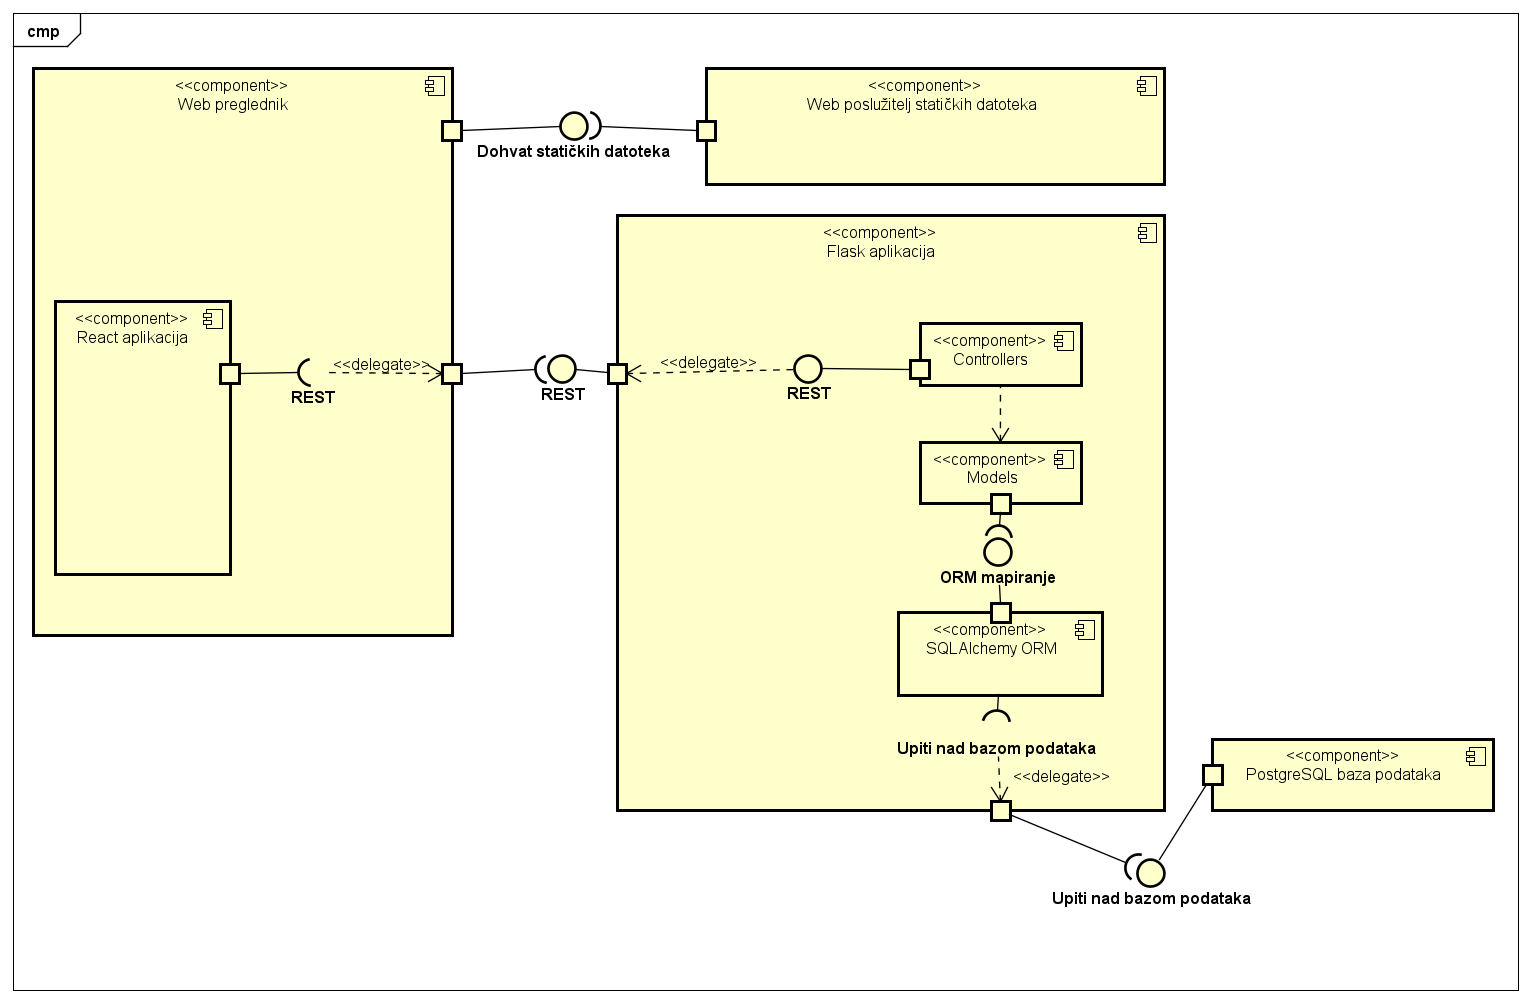
\includegraphics[scale=0.3]{slike/Dijagram_komponenti_Aplikacija.PNG} %veličina slike u odnosu na originalnu datoteku i pozicija slike
				\centering
				\caption{Dijagram komponenti}
				\label{fig:dijagram_komponenti1}
			\end{figure}
			 
			 
			 
			 
	\chapter{Implementacija i korisničko sučelje}
		
		
		\section{Korištene tehnologije i alati}
		
			\textbf{\textit{dio 2. revizije}}
			
			 \textit{Detaljno navesti sve tehnologije i alate koji su primijenjeni pri izradi dokumentacije i aplikacije. Ukratko ih opisati, te navesti njihovo značenje i mjesto primjene. Za svaki navedeni alat i tehnologiju je potrebno \textbf{navesti internet poveznicu} gdje se mogu preuzeti ili više saznati o njima}.
			
			
			\eject 
		
	
		\section{Ispitivanje programskog rješenja}
			
			\textbf{\textit{dio 2. revizije}}\\
			
			 \textit{U ovom poglavlju je potrebno opisati provedbu ispitivanja implementiranih funkcionalnosti na razini komponenti i na razini cijelog sustava s prikazom odabranih ispitnih slučajeva. Studenti trebaju ispitati temeljnu funkcionalnost i rubne uvjete.}
	
			
			\subsection{Ispitivanje komponenti}
			\textit{Potrebno je provesti ispitivanje jedinica (engl. unit testing) nad razredima koji implementiraju temeljne funkcionalnosti. Razraditi \textbf{minimalno 6 ispitnih slučajeva} u kojima će se ispitati redovni slučajevi, rubni uvjeti te izazivanje pogreške (engl. exception throwing). Poželjno je stvoriti i ispitni slučaj koji koristi funkcionalnosti koje nisu implementirane. Potrebno je priložiti izvorni kôd svih ispitnih slučajeva te prikaz rezultata izvođenja ispita u razvojnom okruženju (prolaz/pad ispita). }
			
			
			
			\subsection{Ispitivanje sustava}
			
			 \textit{Potrebno je provesti i opisati ispitivanje sustava koristeći radni okvir Selenium\footnote{\url{https://www.seleniumhq.org/}}. Razraditi \textbf{minimalno 4 ispitna slučaja} u kojima će se ispitati redovni slučajevi, rubni uvjeti te poziv funkcionalnosti koja nije implementirana/izaziva pogrešku kako bi se vidjelo na koji način sustav reagira kada nešto nije u potpunosti ostvareno. Ispitni slučaj se treba sastojati od ulaza (npr. korisničko ime i lozinka), očekivanog izlaza ili rezultata, koraka ispitivanja i dobivenog izlaza ili rezultata.\\ }
			 
			 \textit{Izradu ispitnih slučajeva pomoću radnog okvira Selenium moguće je provesti pomoću jednog od sljedeća dva alata:}
			 \begin{itemize}
			 	\item \textit{dodatak za preglednik \textbf{Selenium IDE} - snimanje korisnikovih akcija radi automatskog ponavljanja ispita	}
			 	\item \textit{\textbf{Selenium WebDriver} - podrška za pisanje ispita u jezicima Java, C\#, PHP koristeći posebno programsko sučelje.}
			 \end{itemize}
		 	\textit{Detalji o korištenju alata Selenium bit će prikazani na posebnom predavanju tijekom semestra.}
			
			\eject 
		
		
		\section{Dijagram razmještaja}
			
			\textbf{\textit{dio 2. revizije}}
			
			 \textit{Potrebno je umetnuti \textbf{specifikacijski} dijagram razmještaja i opisati ga. Moguće je umjesto specifikacijskog dijagrama razmještaja umetnuti dijagram razmještaja instanci, pod uvjetom da taj dijagram bolje opisuje neki važniji dio sustava.}
			
			\eject 
		
		\section{Upute za puštanje u pogon}
		
			\textbf{\textit{dio 2. revizije}}\\
		
			 \textit{U ovom poglavlju potrebno je dati upute za puštanje u pogon (engl. deployment) ostvarene aplikacije. Na primjer, za web aplikacije, opisati postupak kojim se od izvornog kôda dolazi do potpuno postavljene baze podataka i poslužitelja koji odgovara na upite korisnika. Za mobilnu aplikaciju, postupak kojim se aplikacija izgradi, te postavi na neku od trgovina. Za stolnu (engl. desktop) aplikaciju, postupak kojim se aplikacija instalira na računalo. Ukoliko mobilne i stolne aplikacije komuniciraju s poslužiteljem i/ili bazom podataka, opisati i postupak njihovog postavljanja. Pri izradi uputa preporučuje se \textbf{naglasiti korake instalacije uporabom natuknica} te koristiti što je više moguće \textbf{slike ekrana} (engl. screenshots) kako bi upute bile jasne i jednostavne za slijediti.}
			
			
			 \textit{Dovršenu aplikaciju potrebno je pokrenuti na javno dostupnom poslužitelju. Studentima se preporuča korištenje neke od sljedećih besplatnih usluga: \href{https://aws.amazon.com/}{Amazon AWS}, \href{https://azure.microsoft.com/en-us/}{Microsoft Azure} ili \href{https://www.heroku.com/}{Heroku}. Mobilne aplikacije trebaju biti objavljene na F-Droid, Google Play ili Amazon App trgovini.}
			
			
			\eject 
	\chapter{Zaključak i budući rad}
		 
		 Zadatak grupe Proginator bio je izrada aplikacije za medicinsku rehabilitaciju koja omogućava pacijentima prijavljivanje na različite terapije i termine unutar njih, a djelatnicima pregled terapija i evidenciju termina. Nakon 16 tjedana rada u timu ostvarili smo zadani cilj. Projekt se provodio u dvije faze.
		 
		 U prvoj fazi projekta upoznali smo tim i raspravili o znanjima pojedinih članova na temelju čega smo djelomično podijelili zadatke. Također u prvoj fazi raspravili smo što želimo od aplikacije i o tome raspravili s asistentom na temelju čega smo pisali dokumentaciju, posebice obrasce uporabe koji su nam kasnije olakšali implementaciju same aplikacije. Uz dokumentaciju napravili smo i predložak UI dizajna koji je kasnije uvelike pomogao određivanju rasporeda elemenata na korisničkom sučelju i rješavanju nedoumica.
		 
		 U drugoj fazi projekta naglasak je bio na implementaciji aplikacije što je zahtjevalo više samostalnog rada od članova tima. Većina nas se prvi puta susrela sa implementacijom ovakvog projekta što je zahtjevalo dosta samostalnog učenja o korištenim tehnologijama kako bi ostvarili zadane ciljeve. Osim realizacije programskog rješenja u drugoj fazi bilo je potrebno dovršiti dokumentaciju i preostale UML dijagrame kako bi budući korisnici mogli lakše koristiti i vršiti preinake u sustavu. Također bilo je potrebno provesti testiranje. Zbog nekih grešaka u prvom dijelu izrade dokumentacije bilo je potrebno uvesti neke preinake, što je malo usporilo razvoj sustava, ali i dovelo do situacije da nismo implementirali neke funkcionalnosti:
		 \begin{packed_enum}
		 	
		 	\item[-] povezivanje s imenikom liječnika, trenutno imamo samo dodatnu tablicu u bazi koja se ponaša kao imenik liječnika
		 	\item[-] povezivanje s nacionalnim sustavom zdravstvene zaštite, MBO se trenutno provjerava iz dodane tablice u bazi
		 	\item[-] provjera vremena termina i terapija, bilo bi dobro da ima još provjera
		 	\item[-] nije implementiran unos lozinke kod promjene ovlasti djelatnika
		 \end{packed_enum}
		 
		 
		 Redovitim sastancima i komunikacijom preko WhatsAppa i Discorda postigli smo informiranost svih članova grupe o napretku projekta, ali i rješavanje različitih problema koji su se stvorili prilikom implementacije.
		 
		 Trenutno stanje projekta ima podosta mjesta za napredak i dodavanje različitih funkcionalnosti koje bi poboljšale iskustvo korisnika aplikacije, kao i moguća implementacija aplikacije za mobilne uređaje.
		 
		 Sudjelovanje na ovom projektu svim je članovima tima bilo vrijedno iskustvo, ne samo zbog pozitivnih dijelova kao što je usvajanje znanja izrade web aplikacija i dokumentacije, već i onih negativnih, mnogo smo naučili iz pogrešaka koje smo napravili putem, pogotovo što se tiče vremenske organizacije projekta. Zadovoljni smo postignutim bez obzira na puno prostora za napredak.
		 
		 
		 
		 
		  
		 
		 
		
		\eject 
	\chapter*{Popis literature}
		\addcontentsline{toc}{chapter}{Popis literature}
	 	
 		\textbf{\textit{Kontinuirano osvježavanje}}
	
		\textit{Popisati sve reference i literaturu koja je pomogla pri ostvarivanju projekta.}
		
		
		\begin{enumerate}
			
			
			\item  Programsko inženjerstvo, FER ZEMRIS, \url{http://www.fer.hr/predmet/proinz}
			
			\item  The Unified Modeling Language, \url{https://www.uml-diagrams.org/}
			
			\item  Astah Community, \url{http://astah.net/editions/uml-new}
		\end{enumerate}
		
		 
	
	
	\begingroup
	\renewcommand*\listfigurename{Indeks slika i dijagrama}
	%\renewcommand*\listtablename{Indeks tablica}
	%\let\clearpage\relax
	\listoffigures
	%\vspace{10mm}
	%\listoftables
	\endgroup
	\addcontentsline{toc}{chapter}{Indeks slika i dijagrama}


	
	\eject 
		
	\chapter*{Dodatak: Prikaz aktivnosti grupe}
		\addcontentsline{toc}{chapter}{Dodatak: Prikaz aktivnosti grupe}
		
		\section*{Dnevnik sastajanja}
		
		
		\begin{packed_enum}
			\item  sastanak			
			\item[] \begin{packed_item}
				\item Datum: 18. listopada 2023.
				\item Prisustvovali: svi
				\item Teme sastanka:
				\begin{packed_item}
					\item  razjašnjavanje dobivene teme projekta - Medicinska Rehabilitacija
					\item  odabir tehnologija koje će biti korištene u izradi projekta
				\end{packed_item}
			\end{packed_item}
			
			\item  sastanak
			\item[] \begin{packed_item}
				\item Datum: 23. listopada 2023.
				\item Prisustvovali: E.Badurina, L.Lasović, V.Rohak, K.Vrdoljak, F.Zlatar
				\item Teme sastanka:
				\begin{packed_item}
					\item  razjašnjavanje teme projekta
					\item  zapisivanje konkretnih pitanja vezano uz projekt
				\end{packed_item}
			\end{packed_item}
			
			\item  sastanak			
			\item[] \begin{packed_item}
				\item Datum: 25. listopada 2023.
				\item Prisustvovali: svi
				\item Teme sastanka:
				\begin{packed_item}
					\item  podjela uloga
					\item  razrada baze podataka
				\end{packed_item}
			\end{packed_item}
			
			\item  sastanak
			\item[] \begin{packed_item}
				\item Datum: 6. studenoga 2023.
				\item Prisustvovali: svi
				\item Teme sastanka:
				\begin{packed_item}
					\item  komentiranje predloška UI-dizajna
					\item  razrada i dovršavanje baze podataka
					\item  razjašnjavanje dodatnih nejasnoća, pitanja za laboratorijsku vježbu
				\end{packed_item}
			\end{packed_item}
			
			\item  sastanak			
			\item[] \begin{packed_item}
				\item Datum: 8. studenoga 2023.
				\item Prisustvovali: L.Akmačić, E.Badurina, L.Lasović
				\item Teme sastanka:
				\begin{packed_item}
					\item  komentar do sad napravljenog
				\end{packed_item}
			\end{packed_item}
			
			\item  sastanak			
			\item[] \begin{packed_item}
				\item Datum: 15. studenoga 2023.
				\item Prisustvovali: svi
				\item Teme sastanka:
				\begin{packed_item}
					\item  revizija do sada napravljenog
					\item  baza podataka
					\item  funkcionalnost prijave i registracije
				\end{packed_item}
			\end{packed_item}
			
			\item  sastanak			
			\item[] \begin{packed_item}
				\item Datum: 6. prosinca 2024.
				\item Prisustvovali: svi
				\item Teme sastanka:
				\begin{packed_item}
					\item  evaluacija prve verzije projekta
					\item  podjela bodova
					\item  podjela poslova za drugi ciklus
				\end{packed_item}
			\end{packed_item}
			
			\item  sastanak			
			\item[] \begin{packed_item}
				\item Datum: 4. siječnja 2024.
				\item Prisustvovali: svi
				\item Teme sastanka:
				\begin{packed_item}
					\item  predstavljanje do sad napravljenog
					\item  komentiranje dijelova stranice
				\end{packed_item}
			\end{packed_item}
			
			\item  sastanak			
			\item[] \begin{packed_item}
				\item Datum: 10. siječnja 2024.
				\item Prisustvovali: svi
				\item Teme sastanka:
				\begin{packed_item}
					\item  predstavljanje alfa inačice
					\item  podjela preostalog posla
					\item  dogovaranje rokova
				\end{packed_item}
			\end{packed_item}
			
		\end{packed_enum}
		
		\eject
		\section*{Tablica aktivnosti}
		
			\textbf{\textit{Kontinuirano osvježavanje}}\\
			
			 \textit{Napomena: Doprinose u aktivnostima treba navesti u satima po članovima grupe po aktivnosti.}

			\begin{longtblr}[
					label=none,
				]{
					vlines,hlines,
					width = \textwidth,
					colspec={X[7, l]X[1, c]X[1, c]X[1, c]X[1, c]X[1, c]X[1, c]X[1, c]}, 
					vline{1} = {1}{text=\clap{}},
					hline{1} = {1}{text=\clap{}},
					rowhead = 1,
				} 
			
				\SetCell[c=1]{c}{} & \SetCell[c=1]{c}{\rotatebox{90}{\textbf{Ema Badurina}}} & \SetCell[c=1]{c}{\rotatebox{90}{\textbf{Lovro Akmačić }}} &	\SetCell[c=1]{c}{\rotatebox{90}{\textbf{Andrea Jakovčević }}} & \SetCell[c=1]{c}{\rotatebox{90}{\textbf{Lucija Lasović }}} &	\SetCell[c=1]{c}{\rotatebox{90}{\textbf{Vlatko Rohak }}} & \SetCell[c=1]{c}{\rotatebox{90}{\textbf{Karlo Vrdoljak }}} &	\SetCell[c=1]{c}{\rotatebox{90}{\textbf{Fran Zlatar }}} \\  
				Upravljanje projektom 		&  &  &  &  &  &  & \\ 
				Opis projektnog zadatka 	& 4 & 2 & 2 & 2 & 2 & 2 & 2 \\ 
				
				Funkcionalni zahtjevi       & 15 &  &  & 5 &  &  &  \\ 
				Opis pojedinih obrazaca 	& 5 &  &  & 5 &  &  &  \\ 
				Dijagram obrazaca 			& 2 &  & 3 &  &  &  &  \\ 
				Sekvencijski dijagrami 		& 12 &  &  & 4 &  &  &  \\ 
				Opis ostalih zahtjeva 		& 1 &  &  & 1 &  &  &  \\ 

				Arhitektura i dizajn sustava	 &  &  &  & 2 &  &  &  \\ 
				Baza podataka				& 2 & 2 & 2 & 6 & 2 & 3 & 3   \\ 
				Dijagram razreda 			& 3 & 4 &  &  &  &  &   \\ 
				Dijagram stanja				&  &  &  & 5 &  &  &  \\ 
				Dijagram aktivnosti 		&  &  &  & 7 &  &  &  \\ 
				Dijagram komponenti			&  &  &  & 4 &  &  &  \\ 
				Korištene tehnologije i alati 		&  &  &  & 3 &  &  &  \\ 
				Ispitivanje programskog rješenja 	&  &  &  &  &  & 3 &  \\ 
				Dijagram razmještaja			&  &  &  & 2 &  &  &  \\ 
				Upute za puštanje u pogon 		&  &  &  &  &  &  & 0.5 \\  
				Dnevnik sastajanja 			& 0.3 &  &  &  &  &  &  \\ 
				Zaključak i budući rad 		& 2 &  &  &  &  &  &  \\  
				Popis literature 			&  &  &  &  &  &  &  \\  
				&  &  &  &  &  &  &  \\ \hline 
				UI dizajn 			&  &  &  &  & 6 &  &  \\ 
				\textit{Frontend} (prijava i registracija)	&  &  &  &  & 30 &  &  \\ 
				\textit{Frontend} (stranice pacijenta)	&  &  & 50 &  &  &  &  \\ 
				\textit{Frontend} (stranice djelatnika)	& 2 & 60 &  &  &  &  &  \\ 
				\textit{Frontend} (stranice administratora)	&  &  &  &  & 30 &  &  \\ 
				\textit{Frontend} (komponenta za tablice) &  &  &  &  & 30 &  &  \\
				Izrada baze podataka 			&  &  &  &  &  &  & 10 \\ 
				Spajanje s bazom podataka 			&  &  &  &  &  & 5 & 5 \\
				\textit{Backend} (prijava i registracija/ računi(accounts)) 	&  &  &  &  &  & 10 & 10 \\ 
				\textit{Backend} (termini) 	& 3 &  &  &  &  & 17 & 4 \\
				\textit{Backend} (terapije) 	&  &  &  &  &  & 8 & 5 \\
				\textit{Backend} (verifikacija) 	&  &  &  &  &  &  & 20 \\
				\textit{Backend} (sobe) 	&  &  &  &  &  & 5 & 5 \\
				\textit{Backend} (inventar) 	&  &  &  &  &  & 5 & 5 \\
				Deploy	 			&  &  &  &  & 4 & 4 & 14 \\ 
				Ispitivanje aplikacije	 			& 3 & 3 & 3 & 3 & 3 & 3 & 3 \\ 
				Testiranje aplikacije		&  &  &  &  &  & 6 &  \\   
				 							&  &  &  &  &  &  &\\ 
			\end{longtblr}
					
					
		\eject
		\section*{Dijagrami pregleda promjena}
		
		\textbf{\textit{dio 2. revizije}}\\
		
		\textit{Prenijeti dijagram pregleda promjena nad datotekama projekta. Potrebno je na kraju projekta generirane grafove s gitlaba prenijeti u ovo poglavlje dokumentacije. Dijagrami za vlastiti projekt se mogu preuzeti s gitlab.com stranice, u izborniku Repository, pritiskom na stavku Contributors.}
		
	


\end{document} %naredbe i tekst nakon ove naredbe ne ulaze u izgrađen dokument 


